\chapter{Cở sở lý thuyết} \label{chapter02}

\section{Một số loại bệnh trên lá cam}
Trong phần này, chúng tôi giới thiệu mô hình của một chiếc lá để có thể phân loại các bệnh chính xác nhờ đó giúp cho mô hình huấn luyện được chính xác hơn. Tiếp theo, chúng tôi sẽ giới thiệu qua các đặc điểm của từng loại bệnh (Ghẻ nhám, Rầy phấn trắng, Vàng lá gân xanh và Vàng lá thối rễ). Mô hình của một chiếc lá gồm 8 thành phần: (1) Chóp lá, (2) Gân chính, (3) Gân phụ, (4) Phiến lá, (5) Rìa lá, (6) Cuốn lá, (7) Chồi và (8) Thân, được mô tả trong hình \ref{fig:leaf-diagram}.

\begin{figure}[h]
	\centering
	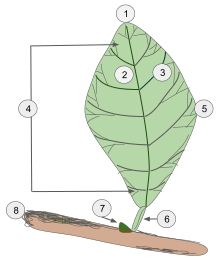
\includegraphics[width=0.4\textwidth]{leaf-diagram}
	\caption[Mô hình của một chiếc lá]{Mô hình của một chiếc lá (Nguồn: wikipedia.org)}
	\label{fig:leaf-diagram}
\end{figure}

Trong đề tài, chúng tôi dùng các ảnh chụp bị nhiễm bốn loại bệnh:
\begin{enumerate}
	\item[-] \emph{Ghẻ nhám}: Nguyên nhân, do nấm. Hiện tượng, vết bệnh đầu tiên là những chấm nhỏ mất màu, trong mờ nhô ra ở mặt dưới lá, sau đó biến thành các mụn nhỏ như mụn ghẻ, màu nâu (hình \ref{fig:benh-ghe-nham}).
	
\begin{figure}[h]
	\centering
	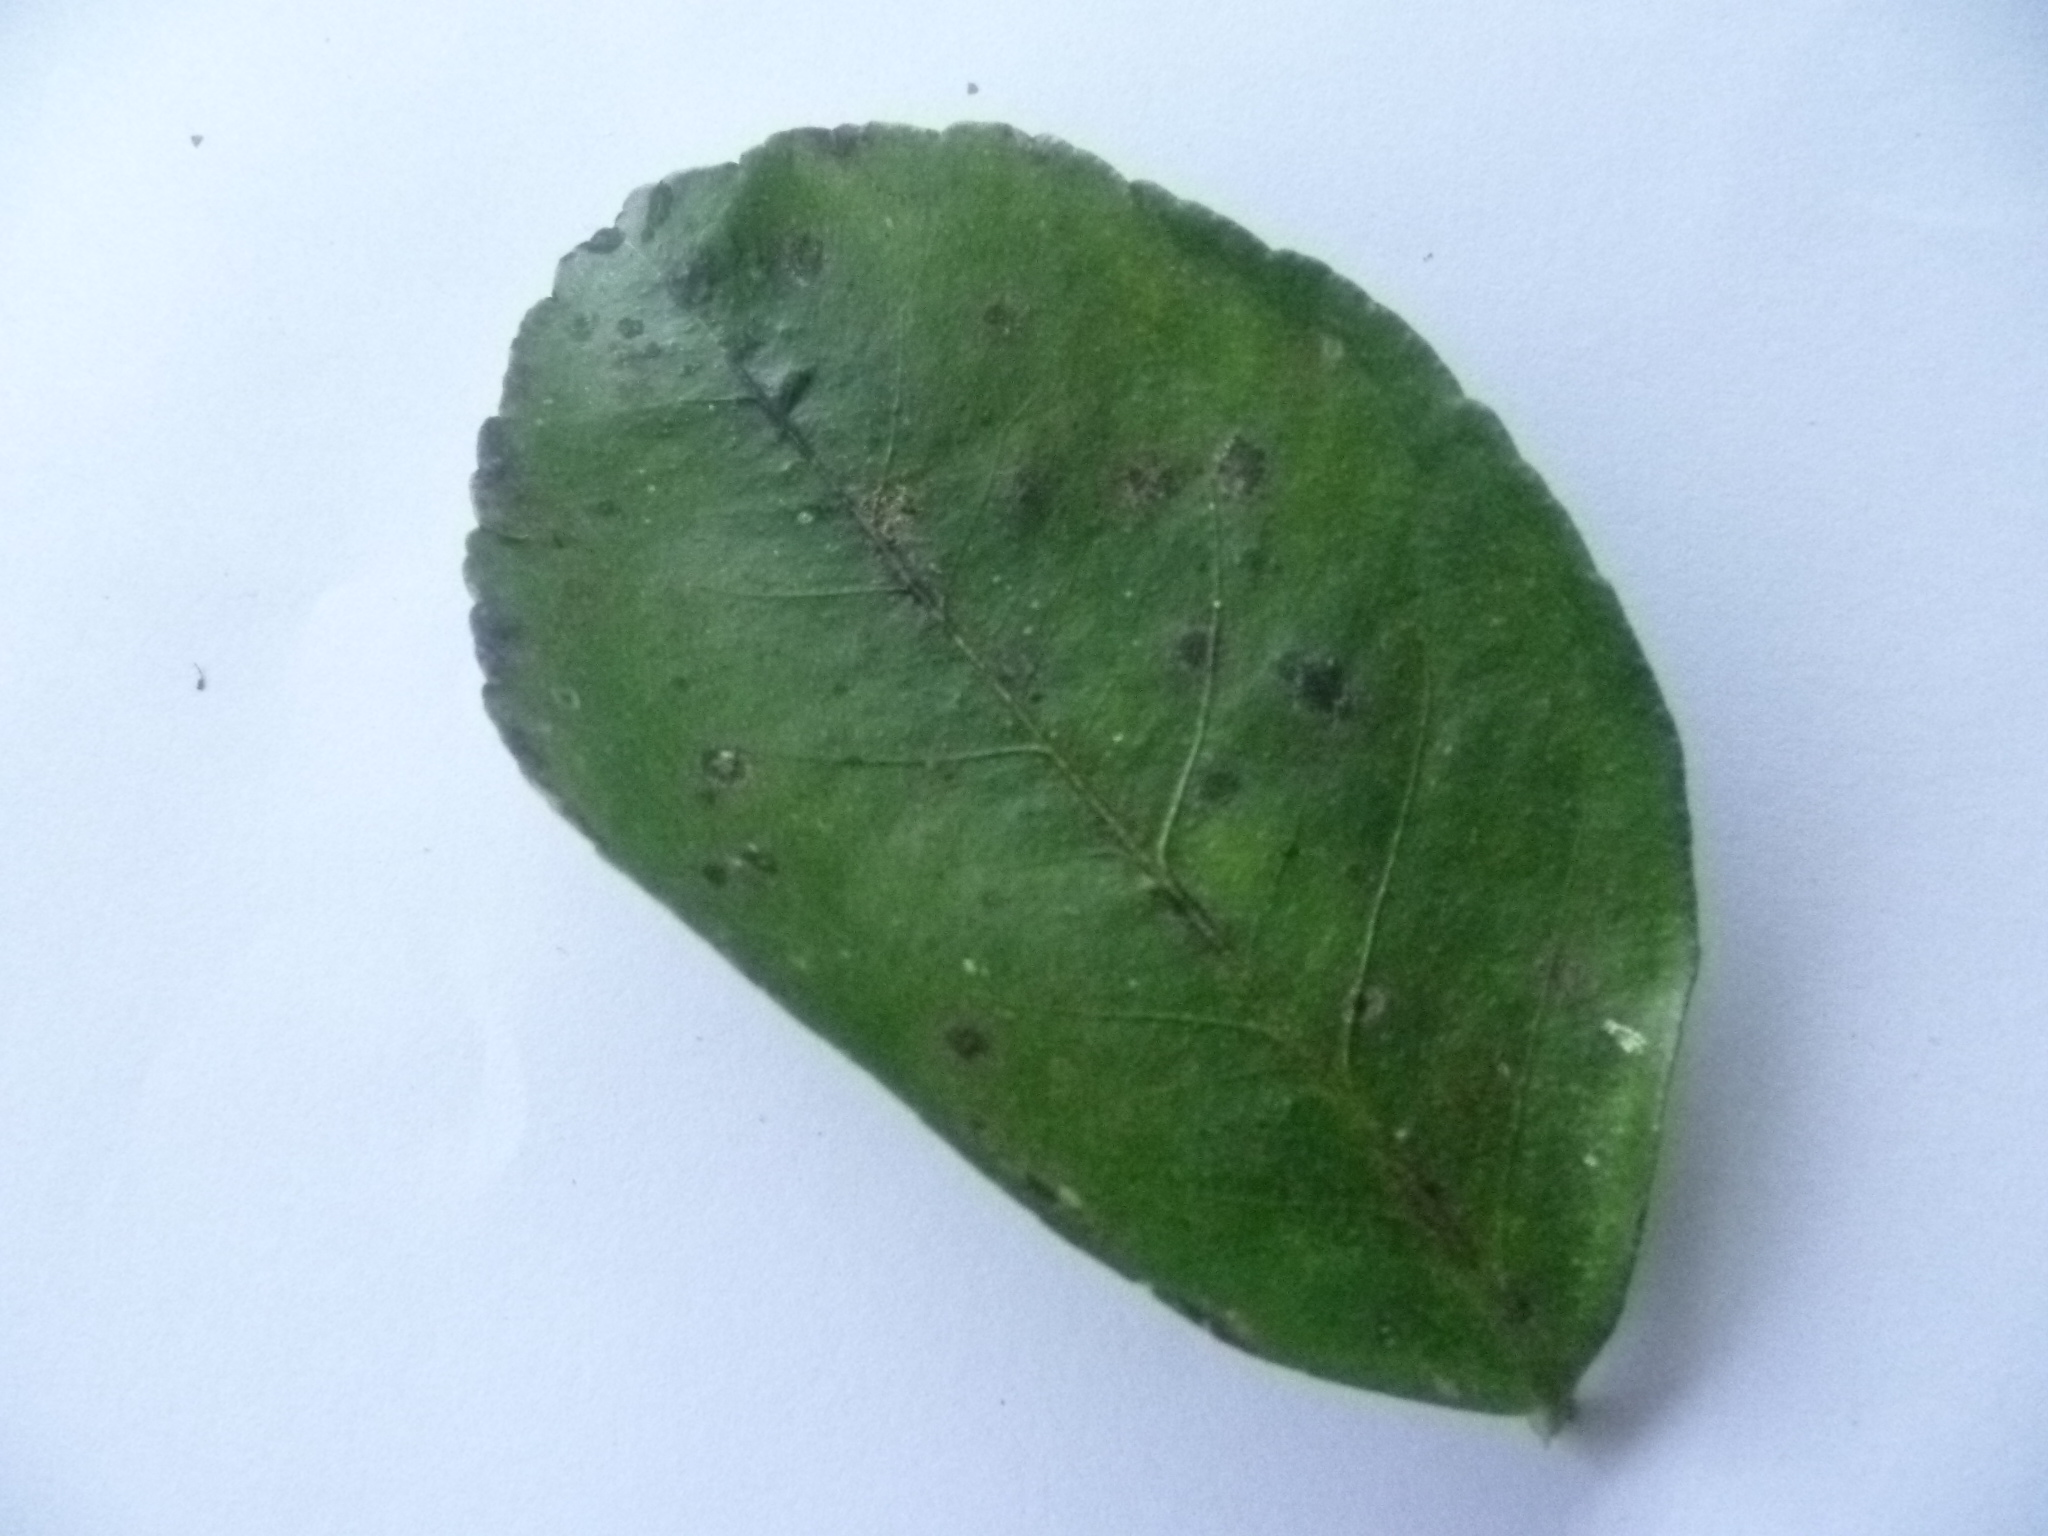
\includegraphics[width=0.4\textwidth]{ghenham}
	\caption{Bệnh Ghẻ nhám}
	\label{fig:benh-ghe-nham}
\end{figure}	
	
	\item[-] \emph{ Rầy phấn trắng}: Nguyên nhân, do rầy đẻ trứng. Hiện tượng, rầy phấn trắng đẻ trứng ở mặt dưới lá, rãi rác thành vòng tròn hình xoắn ốc và được che phủ bởi những lông sáp trắng mịn, mỗi vòng xoắn có khoảng 15 đến 25 trứng (hình \ref{fig:benh-ray-phan-trang}).
	
\begin{figure}[h]
	\centering
	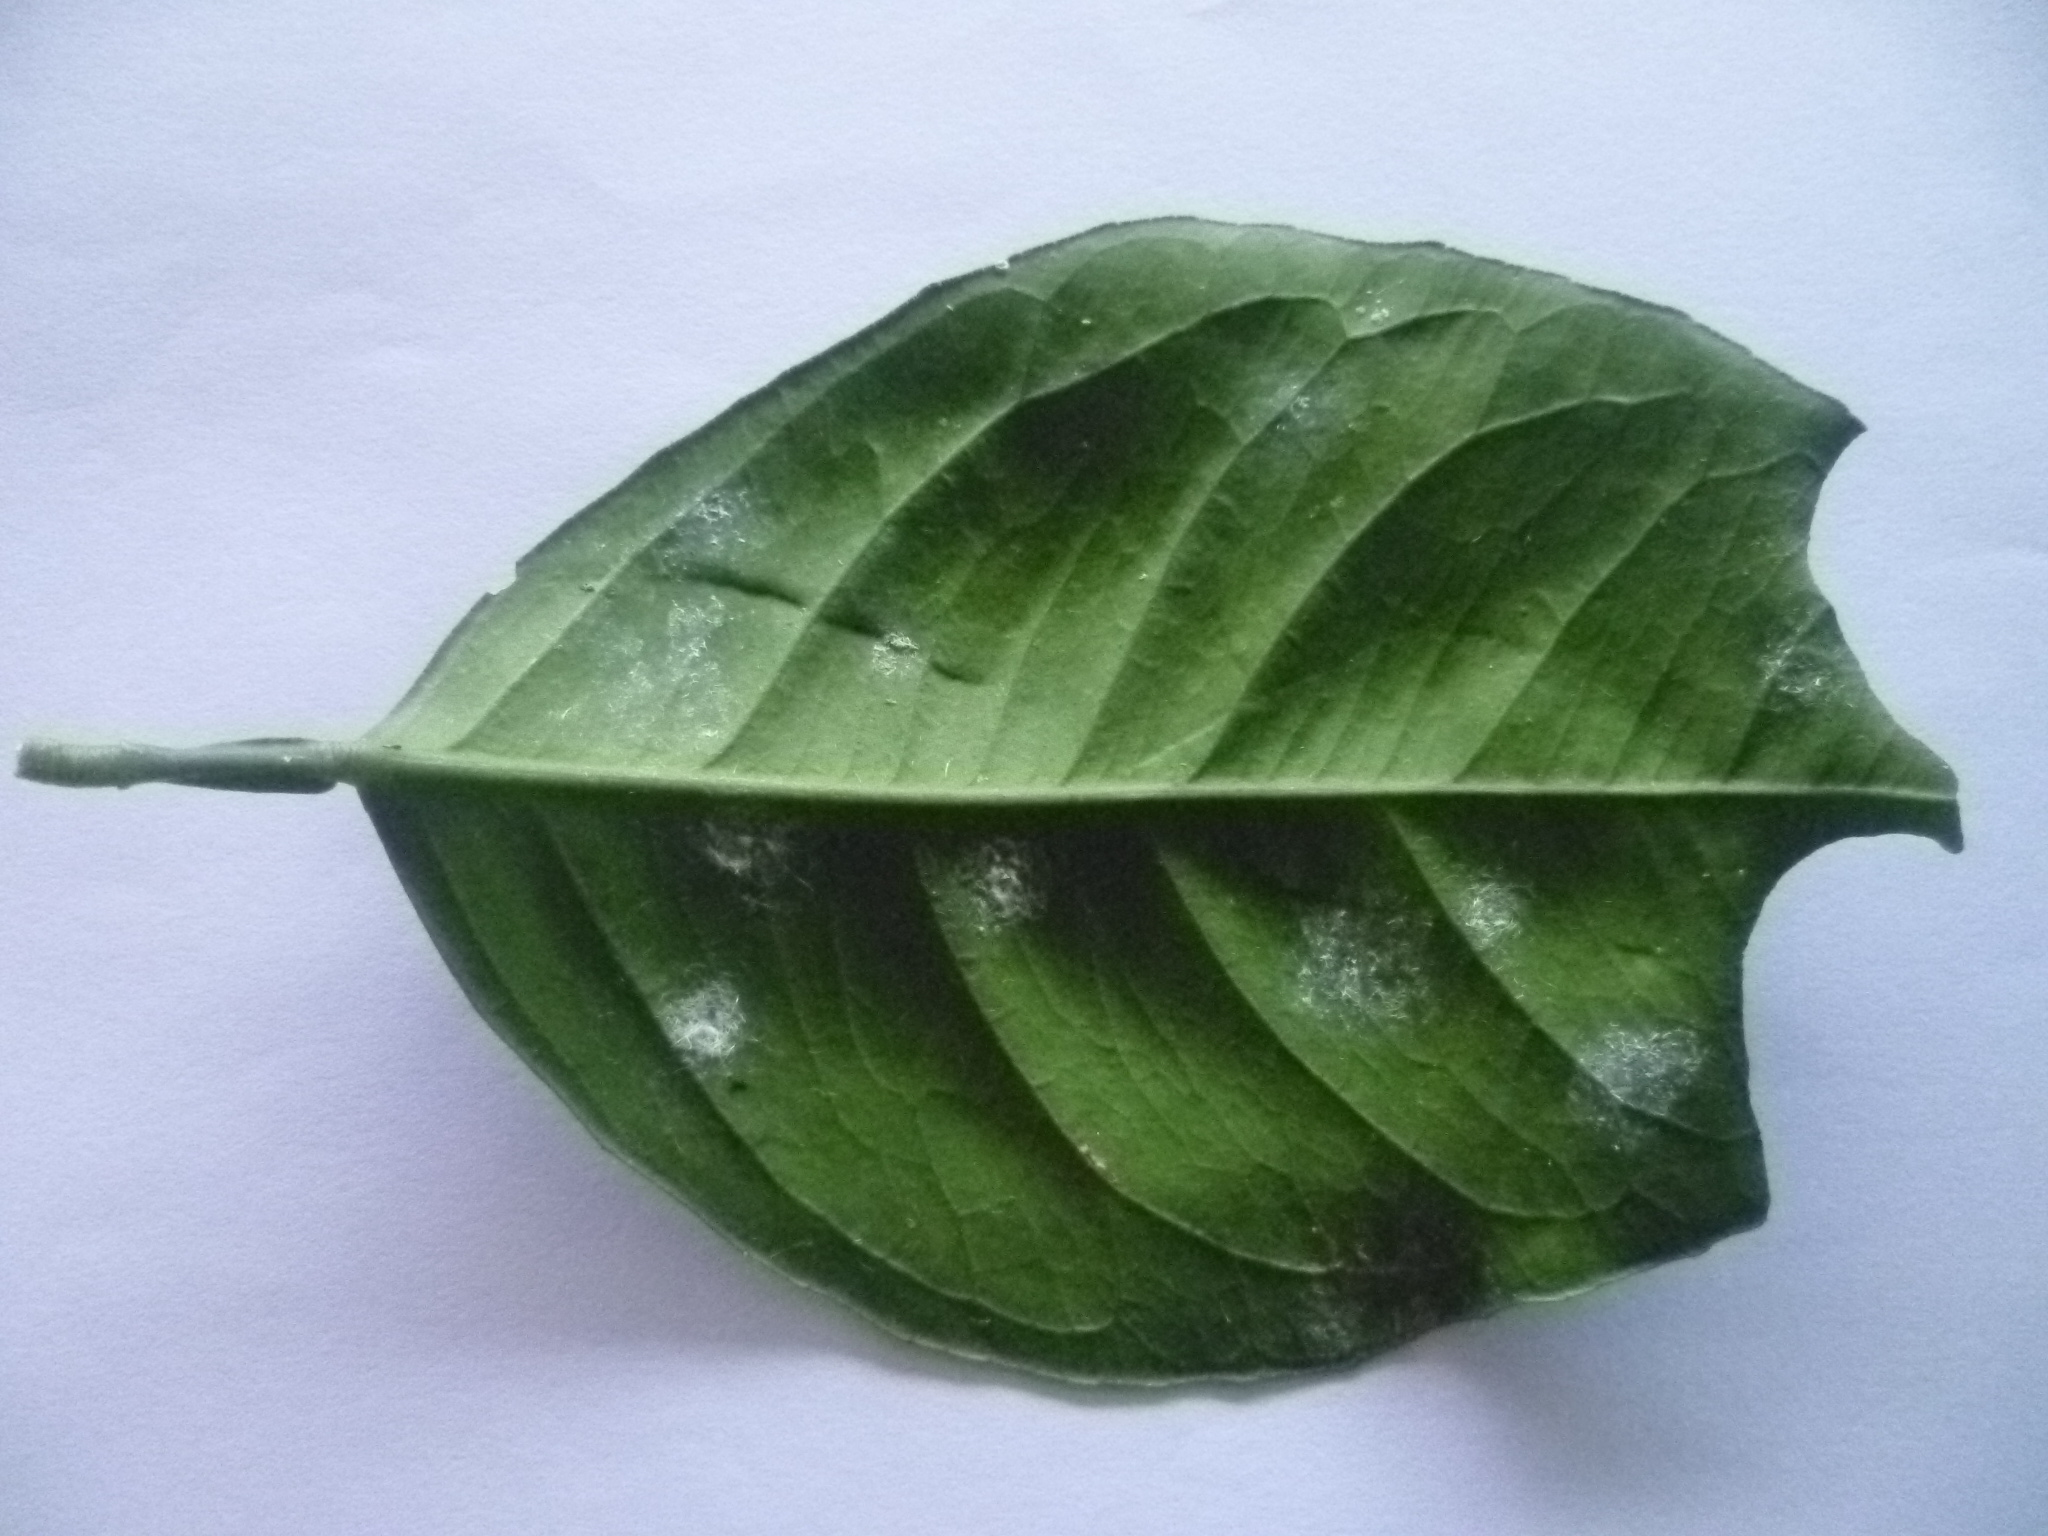
\includegraphics[width=0.4\textwidth]{rayphantrang}
	\caption{Bệnh Rầy phấn trắng}
	\label{fig:benh-ray-phan-trang}
\end{figure}		
	
	\item[-] \emph{Vàng lá gân xanh}: Nguyên nhân, do vi khuẩn. Hiện tượng, phiến lá hẹp, nhọn như hình tai thỏ, khoảng các lá ngắn, lá vàng nhưng gân chính và gân phụ vẫn xanh (hình \ref{fig:benh-vang-la-gan-xanh}).
	
\begin{figure}[!h]
	\centering
	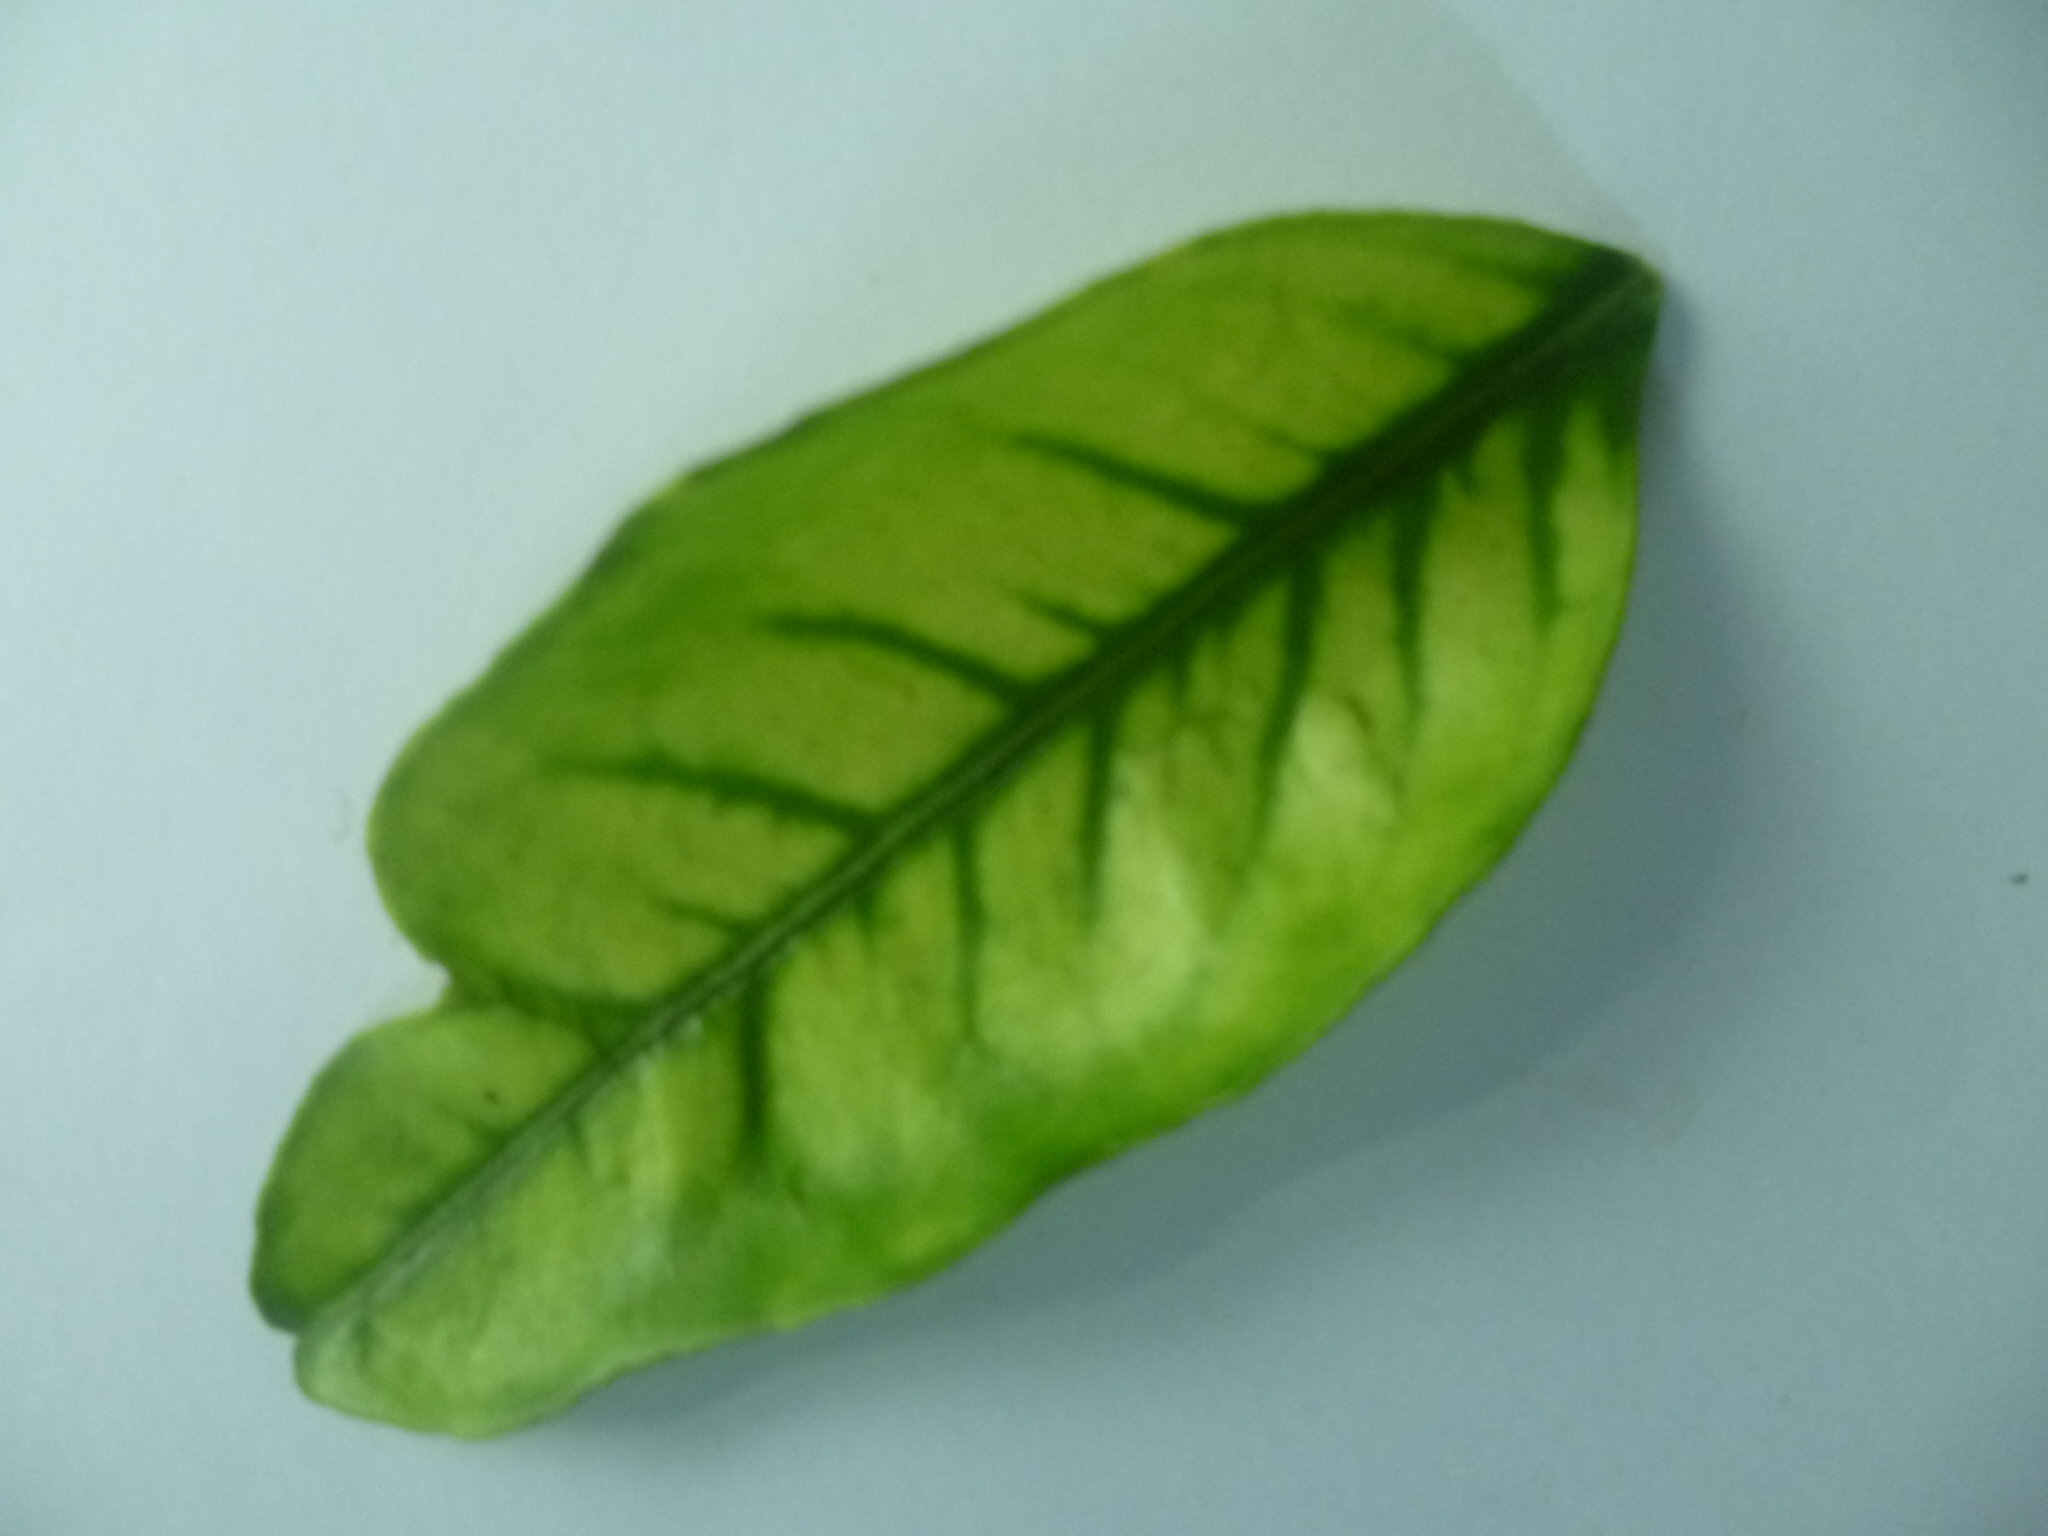
\includegraphics[width=0.4\textwidth]{vanglaganxanh}
	\caption{Bệnh Vàng lá gân xanh}
	\label{fig:benh-vang-la-gan-xanh}
\end{figure}		
	
	\item[-] \emph{Vàng lá thối rễ}: Nguyên nhân, tuyến trùng, rệp sáp đất và nhện hại rễ. Hiện tượng, gân lá màu vàng nhạt, phiến lá ngã vàng cam và dễ rụng (hình \ref{fig:benh-vang-la-thoi-re}).
	
\begin{figure}[h]
	\centering
	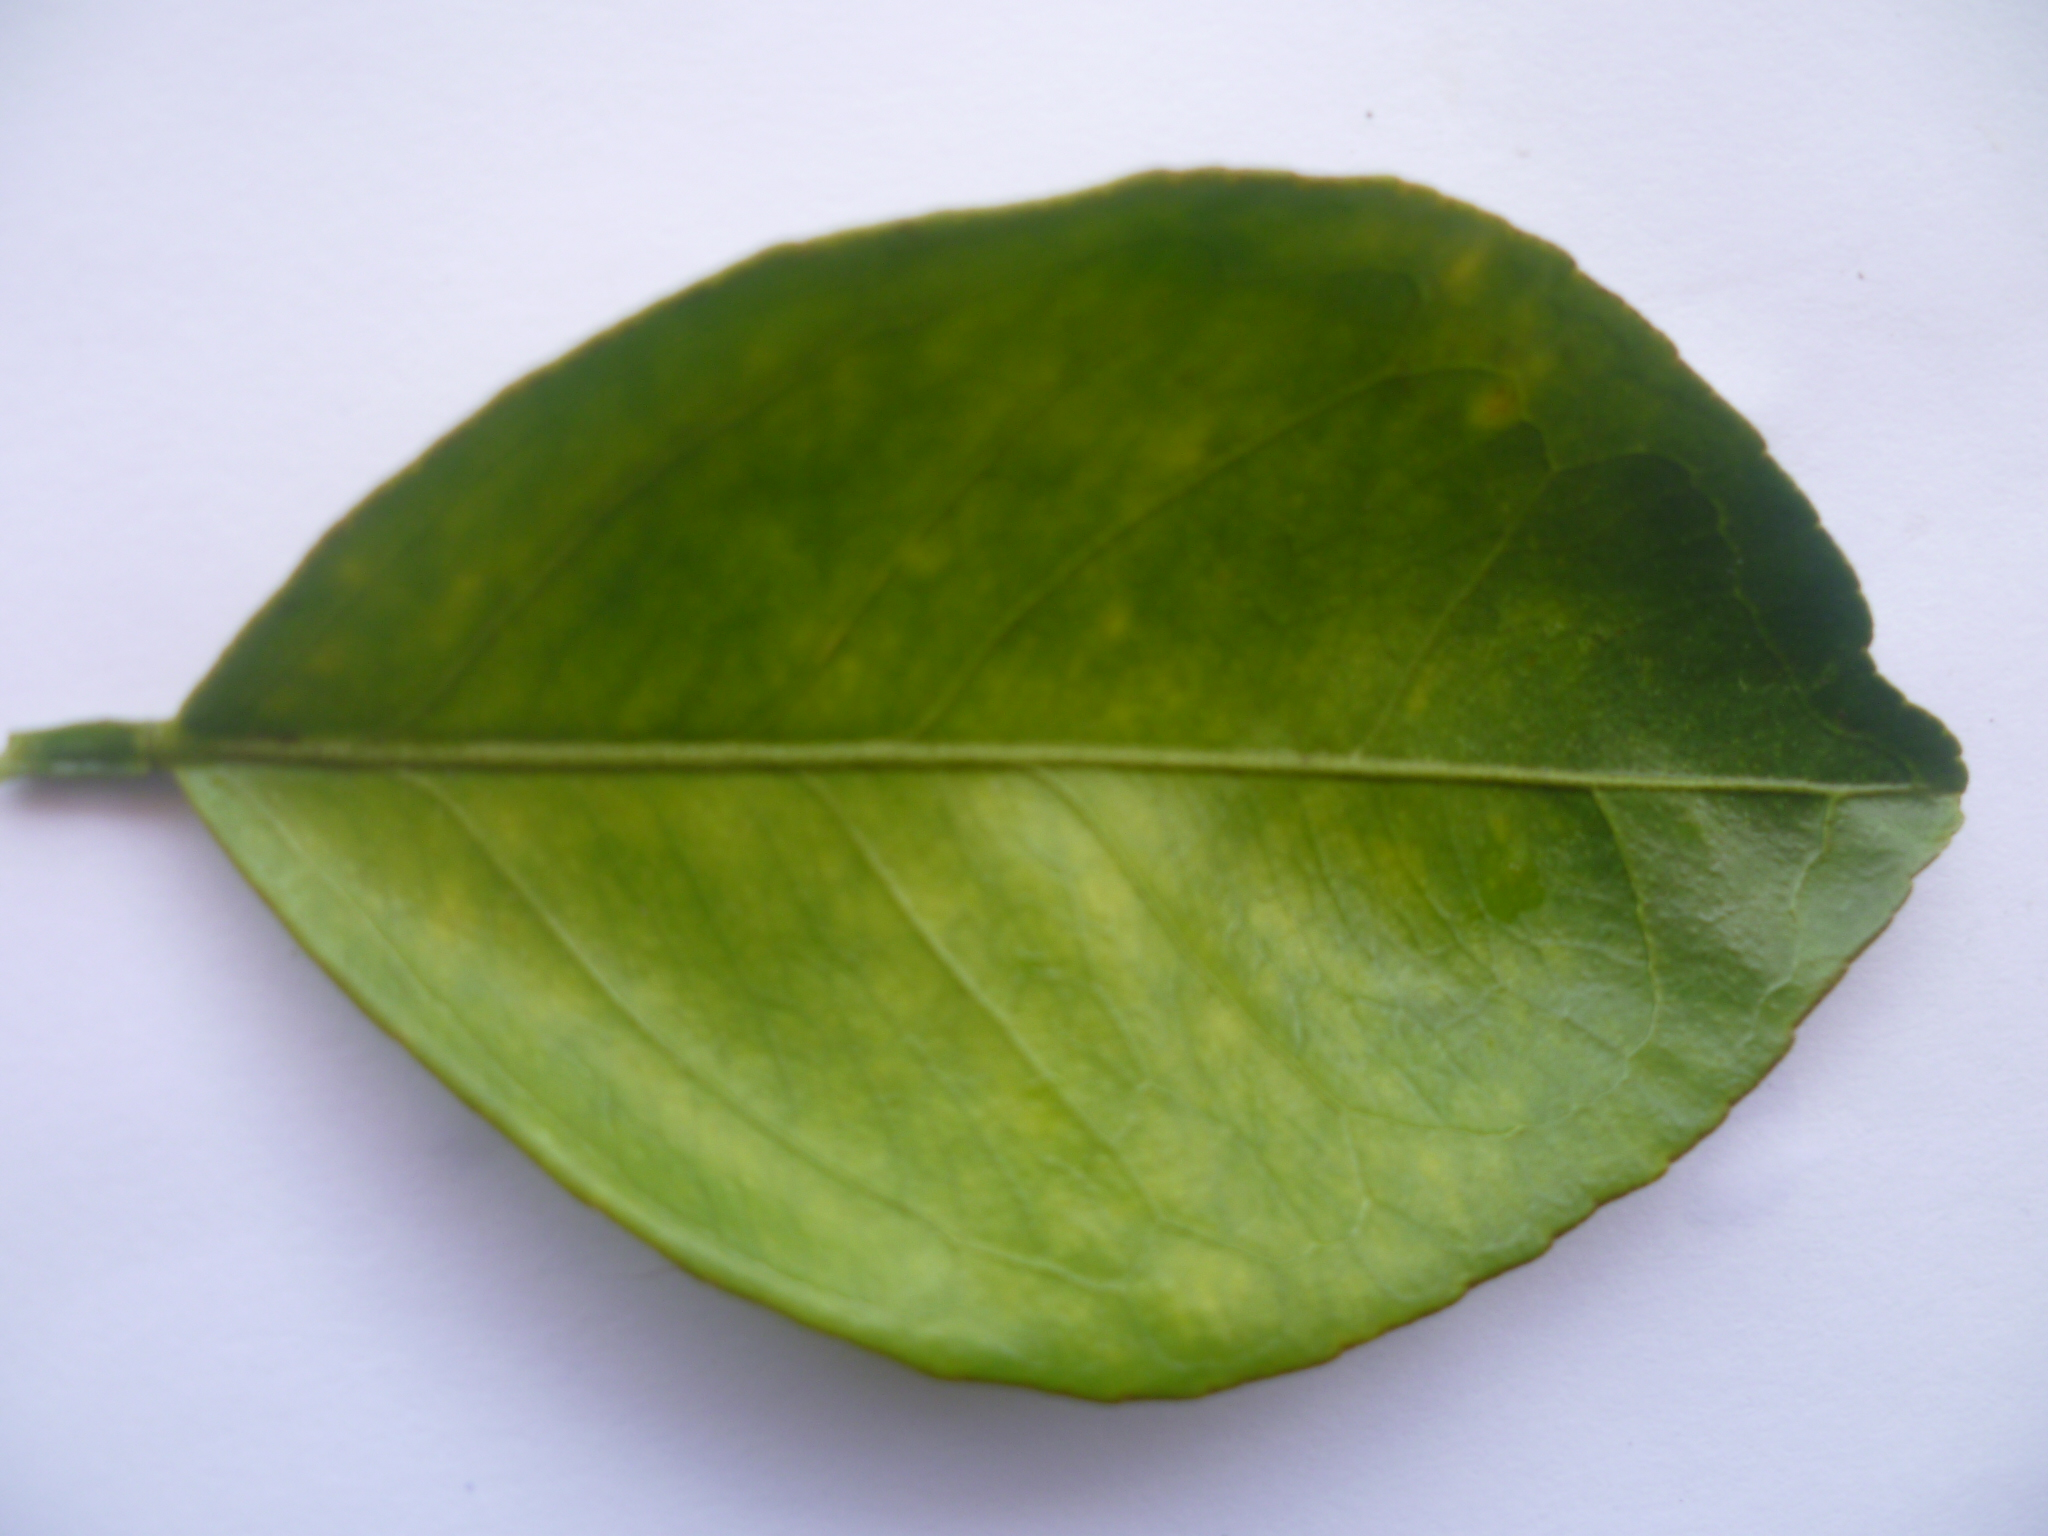
\includegraphics[width=0.4\textwidth]{vanglathoire}
	\caption{Bệnh Vàng lá thối rễ}
	\label{fig:benh-vang-la-thoi-re}
\end{figure}		
	
\end{enumerate}


\section{Các mô hình màu}
\subsection{Giới thiệu}
Phần này giới thiệu về các mô hình màu, vậy màu sắc được định nghĩa như thế nào? Màu sắc là kết quả tương quan giữa ánh sáng (vậy lý) trong môi trường và hệ thống thị giác của con người.\par

Có hai khái niệm cần phân biệt rõ mô hình màu và không gian màu \cite{digitalimageprocessing}:
\begin{itemize}
    \item[-] Mô hình màu là một mô hình toán học trừu tượng mô tả cách màu sắc có thể được biểu thị bằng các bộ số. Ví dụ, RGB, HSV.
    \item[-] Không gian màu là một tổ chức đặc biệt của màu sắc, có thể có các không gian màu khác nhau cho một mô hình màu cụ thể. Ví dụ, sRGB và Adobe RGB là không gian màu của mô hình màu RGB.
\end{itemize}

\subsection{Mô hình màu RGB} \label{subsection-rgb-color-model}
Mô hình màu RGB [RCA, 1953] là một trong những phương pháp biểu diễn màu được sử dụng rộng rãi nhất trong đồ họa máy tính. Nó sử dụng hệ thống tọa độ với ba màu (phốt pho) chính, trong khuôn khổ tài liệu này chúng tôi sẽ dùng ``kênh màu'' thay cho màu. Mỗi kênh màu chính có thể lấy giá trị cường độ từ thấp đến cao (0 -- 1). Trộn ba kênh màu cơ bản này ở các cường độ khác nhau sẽ tạo ra màu sắc khác nhau. Tập hợp tất cả các màu nhận được từ sự kết hợp tuyến tính của các kênh màu đỏ, lục và lam tạo thành mô hình màu RGB hình khối .\par

Trong khối màu RGB như hình \ref{fig:2.1} góc tọa độ tương ứng với màu đen, trong khi góc chéo đối diện là màu trắng. Đường chéo kết nối màu đen và trắng là màu xám. Mô hình màu RGB được dùng cho việc hiển thị lên màu sắc trong các ống tia âm cực, màn hình LCD [Heilmeier, 1986], LED [Holonyack, 1962] và màn hình plasma [Bitzer và Slottow, 1964]. Mỗi điểm ảnh trong màn hình có thể được lưu trong bộ nhớ máy tính như các giá trị độc lập, nó được biến đổi thành các cường độ sáng và gửi đến màn hình. Mỗi điểm ảnh được biểu diễn bằng 3 bytes. Tương ứng 1 byte (1 byte = 8 bits) cho mỗi kênh màu (đỏ, xanh lá cây, xanh dương). Do mã máy là dạng nhị phân (0, 1) nên ta dễ dàng tính được số lượng màu được hiển thị lên một màn hình LCD.
$$ 3(bytes) \times 8(bits) = 24(bits) $$ \par
Số lượng màu được hiển thị trên một màn hình LCD:
$$ 2^{24} = 16.777.216 (color) $$\par

Khi biểu diễn bằng hệ số thập phân (decimal) giá trị nằm trong phạm vi 0 đến 255. Ví dụ, RGB(0,0,0) hoặc rgb(255,255,255). Biểu diễn bằng hệ số thập lục phân (hexadecimal) sẽ bắt đầu bằng dấu \emph{``\#''} chỉ định các giá trị đỏ, lục và lam bằng cách sử dụng 1 đến 4 chữ số hex. Ví dụ, \#RGB, \#rrrrggggbbbb, sử dụng ``\#ffff'' để biểu diễn màu tối đa hoặc ``0'' là không có màu.\par

\begin{figure}[h]
	\centering
	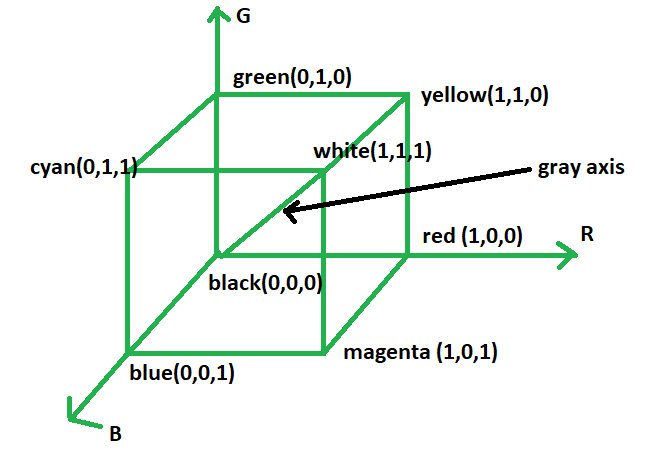
\includegraphics[width=0.6\textwidth]{rgb-color-model}
	\caption[Mô hình màu RGB]{Mô hình màu RGB (Nguồn: wikipedia.org)}
	\label{fig:2.1}
\end{figure}

\subsubsection{Ưu điểm}
Hầu như mọi ứng dụng phổ biến đều tương thích với mô hình màu RGB như Microsoft Office, Adobe Creative Suite (Photoshop, Illustrator, InDesign, v.v) và các trình soạn thảo khác.\par

\subsubsection{Hạn chế}
Một trong những hạn chế chính của mô hình màu RGB là nó không thực sự cho ra màu sắc tốt khi in, việc này dẫn đến sự sai lệch về màu sắc trong các tài liệu được in từ Microsoft Office. Các thiết bị sử dụng loại màn hình LED như Smartphone thì tọa độ màu không được nhất quán. Thậm chí trên cả màn hình TV [Farnsworth, 1927] và một số loại màn hình khác. Vì vậy, giữa các thiết bị khác nhau sẽ có sự sai lệch về màu sắc là khác nhau.\par

\subsection{Mô hình màu HSV}
Ở phần trước \ref{subsection-rgb-color-model} chúng tôi đã nói qua mô hình màu RGB. Không giống như RGB, mô hình màu HSV [Smith, 1978] gần hơn với cách con người cảm nhận màu sắc (bằng mắt).

Mô hình màu HSV gồm có ba thành phần chính Hue, Staturation và Value như hình \ref{fig:2.2}. \emph{Hue} là thành phần màu được biểu thị từ $0^{\circ}$ đến $360^{\circ}$. Đỏ ($0^{\circ}$ -- $60^{\circ}$), Vàng ($61^{\circ}$ -- $120^{\circ}$), Lục ($121^{\circ}$ -- $180^{\circ}$), Lục lam ($181^{\circ}$ -- $240^{\circ}$), Lam ($241^{\circ}$ -- $300^{\circ}$) và Đỏ ($301^{\circ}$ -- $360^{\circ}$). \emph{Saturation} mô tả lượng màu xám (đạm nhạt) của một màu cụ thể, có giá trị 0 đến 100\%, giảm giá trị này về 0 sẽ tạo ra nhiều xám hơn và tạo hiệu ứng mờ dần. Đôi khi, độ được biểu diễn dưới phạm vi 0 đến 1, tương ứng 0 (xám) và 1 (màu chính). \emph{Value} mô tả độ sáng hay cường độ của màu, có giá trị từ 0 đến 100\%, trong đó 0 (đen hoàn toàn) và 100\% (sáng nhất). Một số bộ chọn màu như trong Adobe Photoshop sử dụng thuật ngữ HSB, đó là sự thay thế \emph{B} (bightness) cho \emph{V} (value).

\begin{figure}[h]
	\centering
	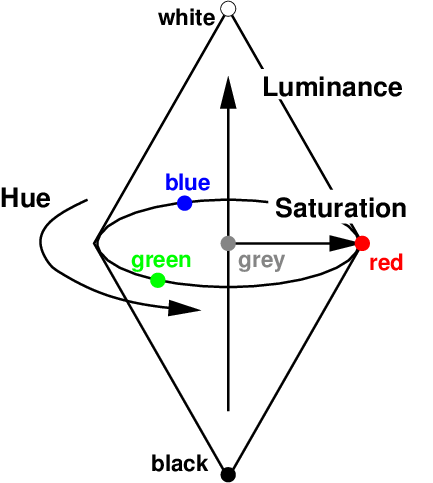
\includegraphics[width=0.4\textwidth]{hsv-color-model}
	\caption[Mô hình màu HSV]{Mô hình màu HSV (Nguồn: researchgate.net)}
	\label{fig:2.2}
\end{figure}

\subsubsection{Ưu điểm}
Mô hình màu HSV có một số ưu điểm tốt hơn so với các mô hình màu khác. Ví dụ, chọn một màu duy nhất trong mô hình màu ABC, nó bỏ qua phần lớn sự phức tạp của màu, nó liên quan về mặt nhận thức đối với tốc độ tính toán, khi các màu này trở nên phức tạp sẽ khó khăn trong việc tính toán. Trong một số ứng dụng đồ họa đều dựa trên mô hình màu RGB. Tuy nhiên, đều cho phép chuyển sang mô hình màu HSV giúp linh hoạt hơn trong lựa chọn màu sản phẩm. Các nhà thiết kế sử dùng mô hình màu HSV khi chọn màu cho sơn hoặc mực vì nó được thể hiện tốt trong mắt người dùng so với mô hình màu RGB.\par

\subsubsection{Hạn chế}
Saturation và Value đã bị giới hạn, do đó thang đo saturation cũng có phạm vi rộng lớn để chứa luôn value. Tương tự RGB, mô hình màu HSV có sự phụ thuộc vào thiết bị hiển thị. Ví dụ: nó có thể chuyển từ màu trắng sang màu lục (xanh lá cây), đó là nhờ sự kết hợp của saturation và value. Màu vàng bão hòa và màu xanh bão hòa có thể được gán cùng một value, nhưng có sự khác biệt lớn về màu sắc đối các hệ thống trong việc kiểm soát giao diện.


\section{Các mô hình biểu diễn ảnh}
\subsection{Giới thiệu}
Ảnh trên máy tính là kết quả thu nhận theo các phương pháp số hóa được nhúng trong các thiết bị kĩ thuật khác nhau camera, scanner, v.v.. Quá trình lưu trữ gồm hai mục đích tiết kiệm bộ nhớ và giảm thời gian xử lý. Việc lưu trữ thông tin trong bộ nhớ có ảnh hưởng rất lớn đến việc hiển thị và in ấn. Việc lưu trữ ảnh được xem như là một tập hợp các điểm ảnh (pixel) cùng kích thước, nếu sử dụng càng nhiều điểm ảnh thì bức ảnh càng đẹp, càng mịn và thể hiện rõ các chi tiết trong ảnh, người ta gọi đặc điểm này là độ phân giải. Việc lựa chọn độ phân giải thích hợp phụ thuộc vào nhu cầu sử dụng và trặc trưng của mỗi ảnh cụ thể. Trên cơ sơ đó, ảnh thường được biểu diễn theo hai mô hình cơ bản là mô hình raster và mô hình vector.\par

\subsection{Mô hình raster}
Đây là cách biểu diễn thông dụng nhất hiện nay, ảnh được biểu diễn dưới dạng ma trận các điểm ảnh như hình \ref{fig:2.3}. Thường được thu nhận qua các thiết bị camera, scanner, v.v. tùy theo yêu cầu mà mỗi điểm ảnh được biểu diễn bằng một hay nhiều bit.\par
Một trong những hướng nghiên cứu cơ bản trên mô hình biểu diễn này là các kỹ thuật nén ảnh, các kỹ thuật nén ảnh được chia hai khuynh hướng nén bảo toàn và nén không bảo toàn thông tin. Nếu nén bảo toàn có khả năng phục hồi bảo toàn dữ liệu ban đầu, thì nén không bảo toàn chỉ có khả năng phục hồi trong một sai số cho phép nào đó. Theo mô hình này có thể dễ dàng thấy một số ảnh được biểu diễn với phần mở rông như BMP, TIF, GIF, v.v. Mô hình raster thuận lợi cho việc hiển thị và in ấn.

\begin{figure}[h]
	\centering
	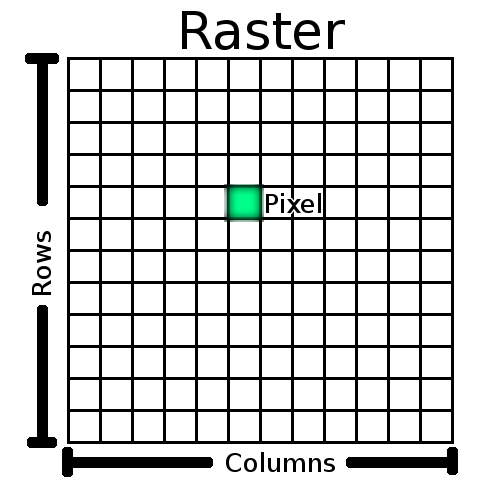
\includegraphics[width=0.3\textwidth]{raster-model}
	\caption[Mô hình biểu diễn ảnh raster]{Mô hình biểu diễn ảnh raster (Nguồn: docs.qgis.org)}
	\label{fig:2.3}
\end{figure}

\subsection{Mô hình vector}
Mô hình vector được sử dụng cho việc biểu diễn ảnh ngoài mục đích tiết kiệm không gian lưu trữ, dễ dàng cho hiển thị, in ấn, sao chép, di chuyển và tìm kiếm.\par

Trong mô hình này, sử dụng hướng giữa các vector của điểm ảnh lân cận như hình \ref{fig:2.4} để mã hóa và tái tạo ảnh. Ban đầu ảnh vector được thu nhận trực tiếp từ các thiết bị kĩ thuật số digital hoặc được chuyển đổi từ ảnh raster thông qua các chưg trình số hóa. Do công nghệ phần cứng đa phần chỉ hỗ trợ cho ảnh raster nên các nghiên cứu về biểu diễn ảnh vector đều tập trung từ chuyển đổi ảnh raster. Có thể thấy sự khác biệt giữa hai cách biểu diễn ảnh trong trong thực tế ở hình \ref{fig:2.5}.\par

\begin{figure}[h]
	\centering
	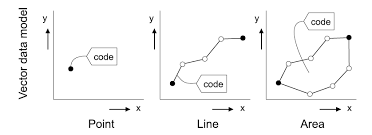
\includegraphics[width=0.6\textwidth]{vector-model}
	\caption[Mô hình biểu diễn ảnh vector]{Mô hình biểu diễn ảnh vector (Nguồn: deltauniv.edu.eg)}
	\label{fig:2.4}
\end{figure}

\begin{figure}[h]
	\centering
	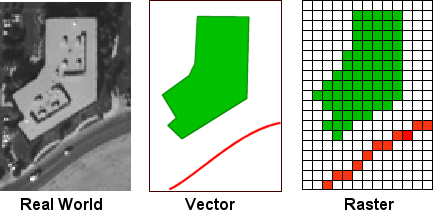
\includegraphics[width=0.5\textwidth]{real-world-vector-raster}
	\caption[Mô hình biểu diễn ảnh vector và raster trong thực tế]{Mô hình vector và raster trong thực tế (Nguồn: geography.hunter.cuny.edu)}
	\label{fig:2.5}
\end{figure}

\subsection{Phân loại ảnh}
\subsubsection{Ảnh nhị phân}
Như tên gọi của nó, ảnh nhị phân (1 bit) một điểm ảnh chỉ chứa một giá trị là 0 hoặc 1. Trong đó, giá trị 0 đại diện cho màu đen và giá trị 1 đại diện cho màu trắng như hình \ref{fig:2.6}, còn gọi là ảnh đơn sắc. Ảnh thu được chỉ bao gồm màu trắng và đen nên còn được gọi là ảnh trắng đen, nó có định dạng PBM (bitmap). Tùy vào độ phân giải của ảnh, có thể biểu diễn bằng một ma trận có kích thước khác nhau, hình \ref{fig:2.6} được biểu diễn bằng một ma trận kích thước 35$\times$35. \par

\begin{figure}[h]
	\centering
	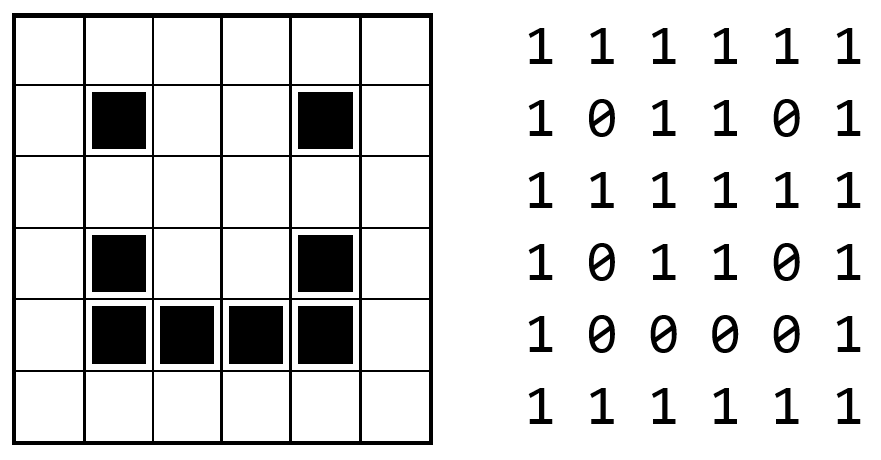
\includegraphics[width=0.4\textwidth]{binary-image}
	\caption[Ảnh nhị phân]{Ảnh nhị phân (Nguồn: thimbleprojects.org)}
	\label{fig:2.6}
\end{figure}

\subsubsection{Ảnh mức xám}
Khác với ảnh nhị phân được biểu diễn bằng 1 bit, ảnh mức xám hay ảnh xám (gray-level) được biểu diễn 8 bits trên mỗi điểm ảnh giá trị nằm trong phạm vi 0 đến 255. Trong đó, 0 (màu đen), 127 (màu xám) và 255 (màu trắng). \par
Định dạng ban đầu được sử bởi các mô hình của hệ điều hành UNIX [Thompson, Ritchie và Mcllroy, 1969] và màu Macintosh [Apple, 1993] đầu tiên. Ảnh mức xám có định dạng PGM khác với ảnh nhị phân (PBM), định dạng này không hỗ trợ mặc đinh trên hệ điều hành Windows. Muỗn xem được trên Windows cần phải có trình xem ảnh hoặc bộ công cụ xử lý ảnh như MATLAB [MathWorks, 1984]. Ảnh mức xám được biểu diễn bằng mô hình raster với một ma trận hai chiều, có giá trị nằm trong khoảng 0 đến 255 (hình \ref{fig:2.7}).\par

\begin{figure}[h]
	\centering
	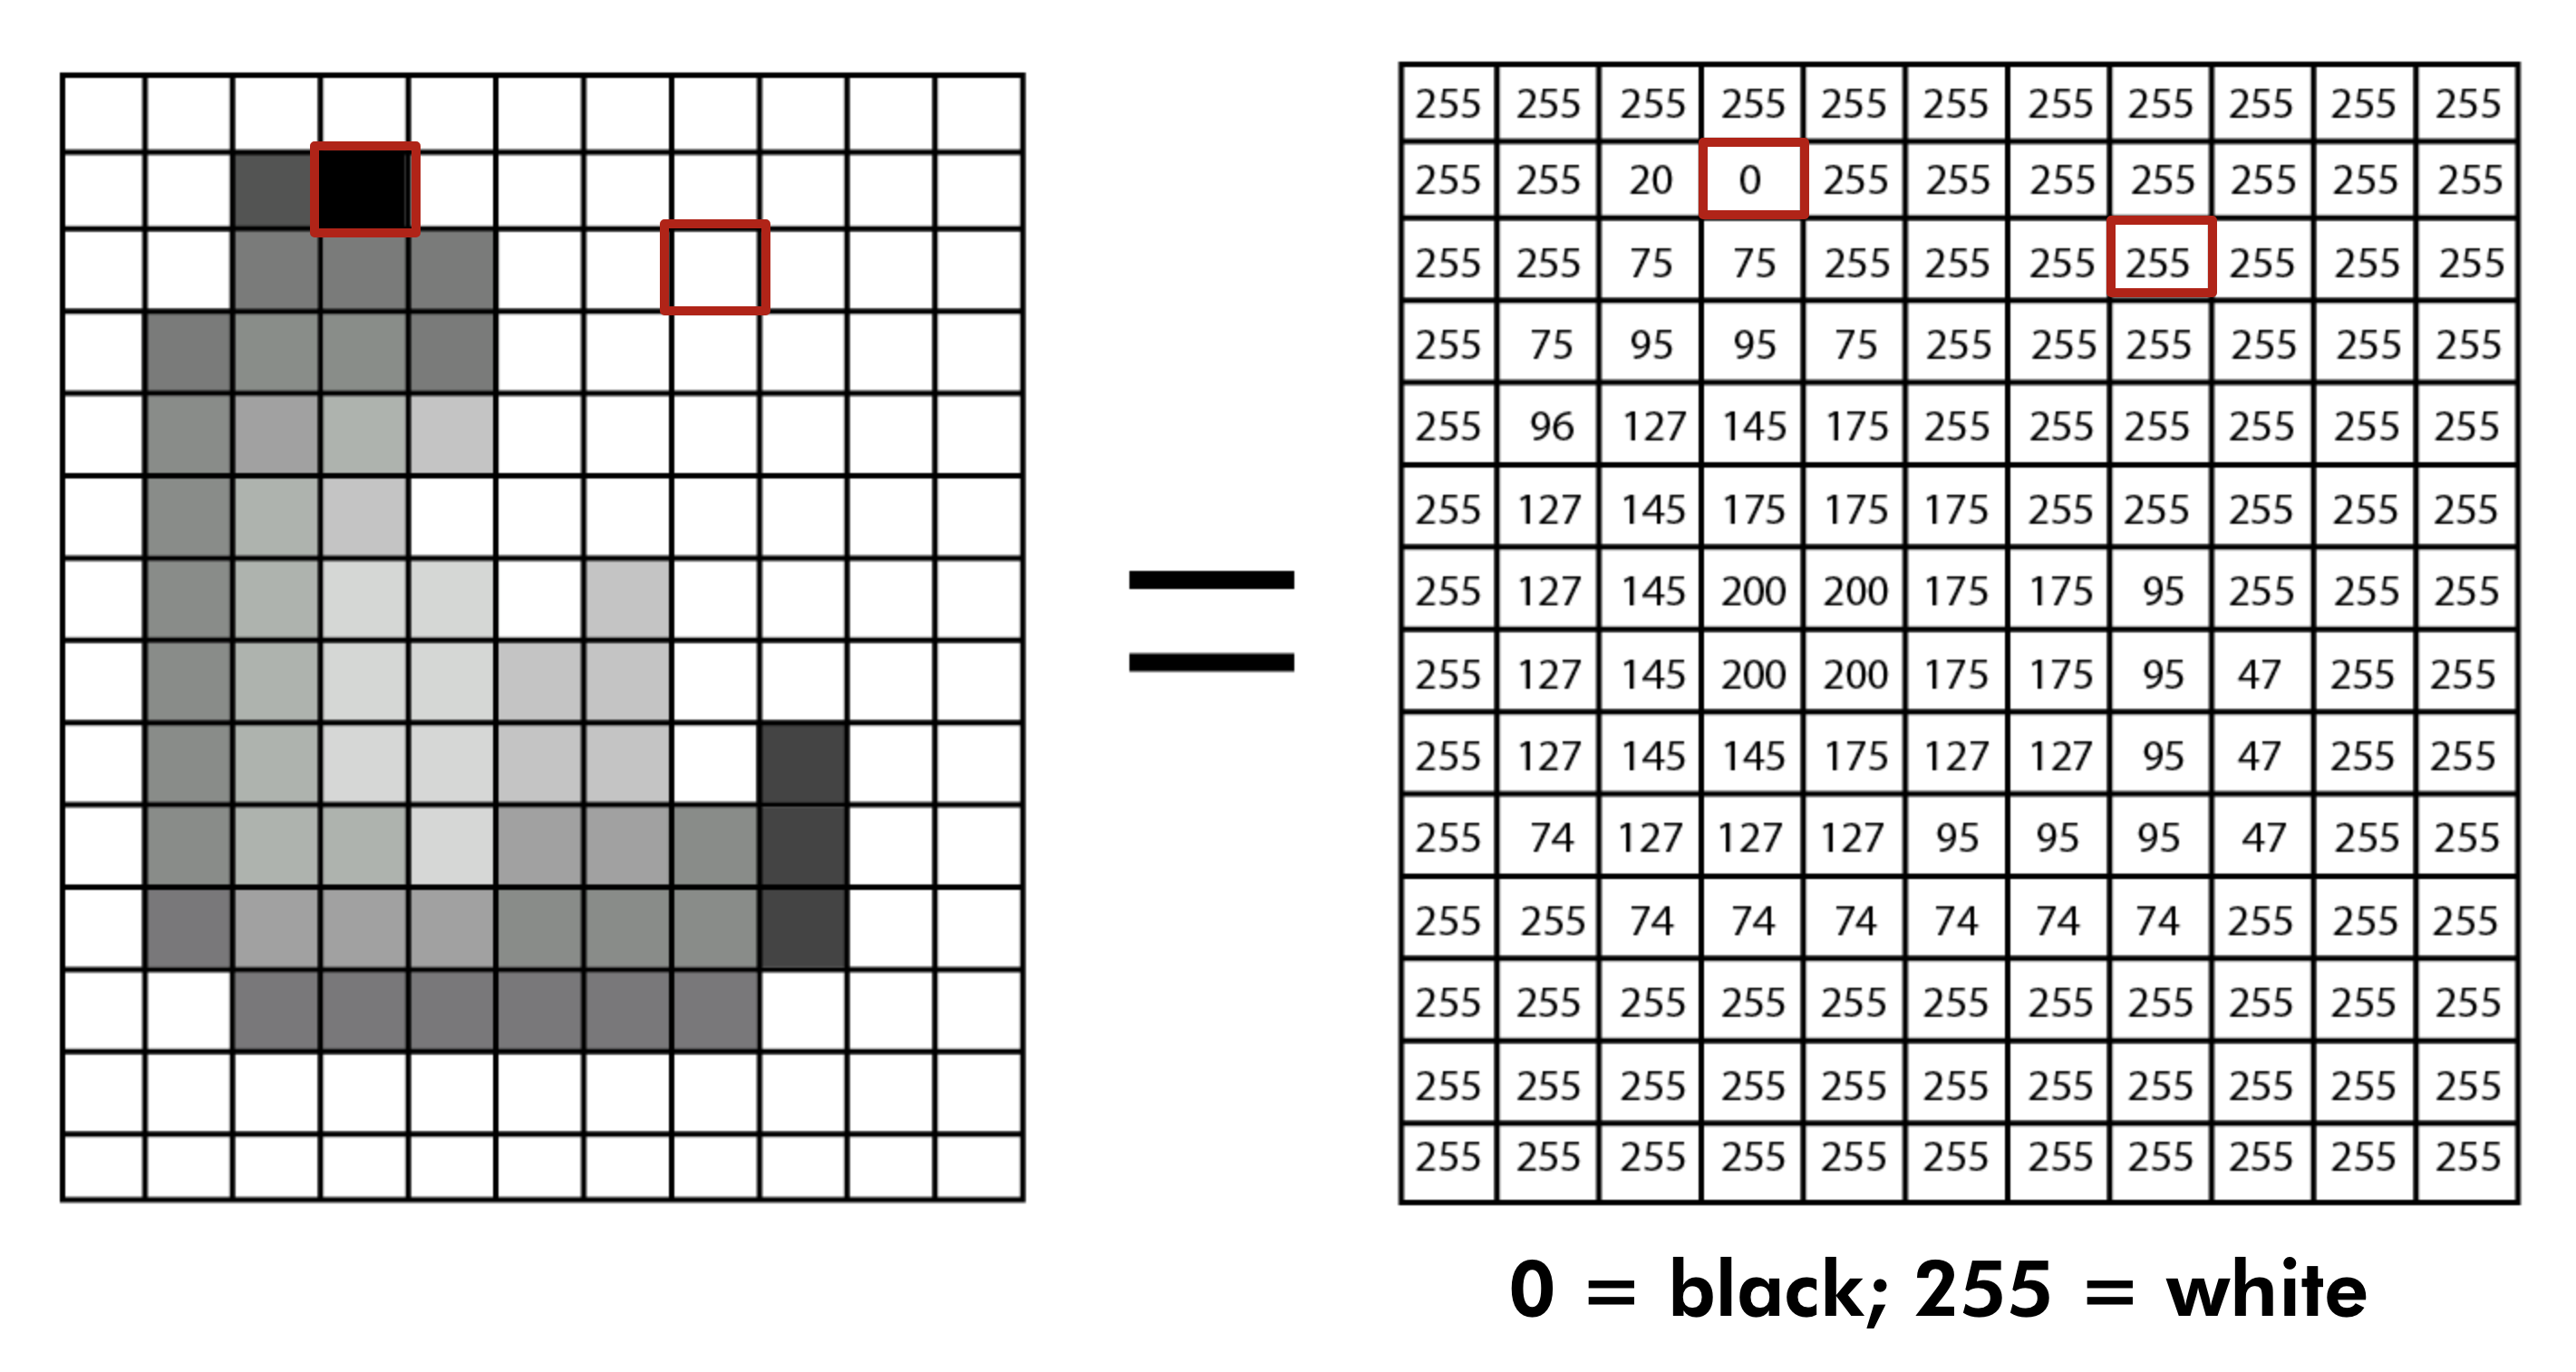
\includegraphics[width=0.7\textwidth]{grayscale-image}
	\caption[Ảnh mức xám]{Ảnh mức xám (Nguồn: edtech.engineering.utoronto.ca)}
	\label{fig:2.7}
\end{figure}

\subsubsection{Ảnh màu}
Ảnh màu là sự phát triển của ảnh mức xám. Có thể biết được nhiều thông tin hơn dựa vào màu sắc, các thông tin này có thể đơn giản hóa dùng cho việc phân tích hình ảnh [7]. Ví dụ, xác định đối tượng hoặc trích xuất đặc trưng của một ảnh dựa trên màu sắc. Màu sắc được xác định dựa vào bước sóng có giá trị lớn hơn các bước sóng còn lại. Màu sắc nhìn thấy được trong khoảng 400nm (tím) và 700 (đỏ) trên phổ điện từ như hình \ref{fig:2.8}.\par

\begin{figure}[!htp]
	\centering
	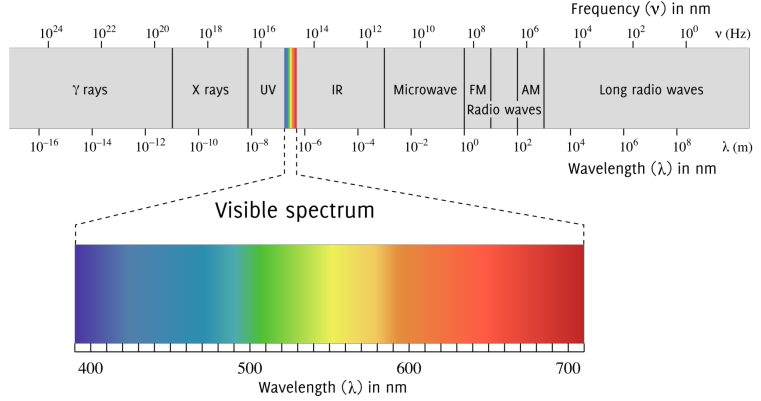
\includegraphics[width=0.7\textwidth]{visible-spectrum}
	\caption[Quang phổ nhìn thấy ở người]{Quang phổ nhìn thấy ở người (Nguồn: inf.edu.ac.uk)}
	\label{fig:2.8}
\end{figure}

Ban đầu ảnh được biểu diễn bằng 16 bits trên mỗi điểm ảnh, tương ứng với 65,356 các màu khác nhau, còn gọi là định dạng màu cao. Giá trị 16 bits được chia thành ba kênh màu (đỏ, xanh lá cây, xanh dương), số lượng bit được chia tương ứng 5 bits, 6 bits và 5 bits.\par

Như chúng tôi đã giới thiệu ở phần \ref{subsection-rgb-color-model} mô hình màu RGB được biểu diễn bằng 24 bits trên mỗi điểm ảnh. Tương tự như cách biểu diễn 16 bits, giá trị 24 bits được chia tương ứng cho ba kênh màu RGB. Có thể thấy trong hình \ref{fig:2.9} mỗi kênh màu được biểu diễn bằng một giá trị 8 bits. Đối với ảnh biểu diễn bằng giá trị 24 bits được sử dụng phổ biến nhất hiện nay, nó có định dạng PPM.\par

\begin{figure}[!htp]
	\centering
	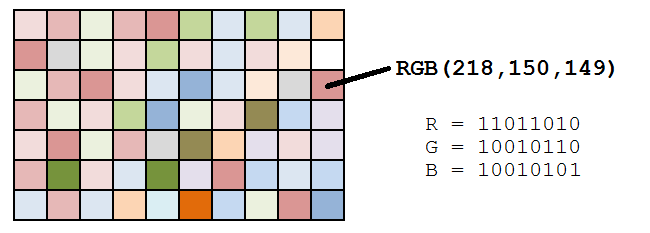
\includegraphics[width=0.6\textwidth]{color-image}
	\caption[Ảnh màu 24 bits]{Ảnh màu 24 bits (Nguồn: towardsdatascience.com )}
	\label{fig:2.9}
\end{figure}


\section{Các phương pháp trích chọn đặc trưng}
\subsection{Giới thiệu}
Trích chọn đặc trưng là cơ sở của tra cứu ảnh dựa vào nội dung. Theo nghĩa rộng, các đặc trưng có thể bao gồm cả các đặc trưng dựa vào văn bản và các đặc trưng trực quan như màu sắc, kết cấu và hình dạng. Trích chọn đặc trưng giúp giảm lượng dữ liệu phải xử lý, trong khi vẫn mô tả chính xác toàn bộ dữ liệu gốc. Quá trình trích chọn đặc trưng là hữu ích, vì nó làm giảm lượng dữ liệu dư thừa nhưng không làm mất thông tin quan trọng hoặc có liên quan giúp tăng thời gian nhận dạng. Tùy vào mục đích xây dựng mô hình nhận dạng mà chọn các kỹ thuật trích chọn đặc trưng sao cho phù hợp.\par

\subsection{Trích chọn đặc trưng SIFT}\label{sub:sift}
Đặc trưng SIFT (Scale-Invariant Feature Transform) [Lowe, 2004] là giải thuật trong nghành Khoa học máy tính, dùng để nhận dạng và miêu tả những điểm đặc trưng cục bộ trong ảnh, được ứng dụng rộng rải trong nhận dạng đối tượng (object recognition), mô hình hóa 3D (3D modeling), v.v.. Đặc trưng cục bộ SIFT không bị thay đổi trước những biến đổi tỉ lệ ảnh, tịnh tiến, phép quay, không bị thay đổi một phần đối với phép biến đổi hình học affine (thay đổi góc nhìn) và mạnh với những thay đổi tỷ lệ về độ sáng, nhiễu và sự che khuất.\par

\emph{Điểm hấp dẫn} (keypoint) là điểm ảnh hấp dẫn trên ảnh, có nghĩa là điểm đó có các đặc trưng bất biến. Trong bài báo khoa học \cite{lowe2004distinctive} giải thuật SIFT trải qua bốn giai đoạn tính toán chính:

\begin{enumerate}
\item Phát hiện điểm cực trị.

\item Định vị điểm hấp dẫn.

\item Xác định hướng cho điểm hấp dẫn.

\item Mô tả các điểm hấp dẫn.
\end{enumerate}

\subsubsection{Phát hiện điểm cực trị}
Các điểm hấp dẫn với đặc trưng SIFT tương thích với các cực trị cục bộ của bộ lộc difference-of-Gaussian (DoG) ở các tỉ lệ khác nhau. Định nghĩa không gian tỉ lệ của một ảnh là hàm $L(x,y,k\sigma)$ là kết quả từ việc nhân chập biến tỉ lệ $G(x,y,k\sigma)$ với ảnh đầu vào $I(x,y)$:
	
\begin{equation}\label{eq:01}
L(x,y,k\sigma) = G(x,y,k\sigma)*I(x,y)
\end{equation}
	
khi đó, $*$ là phép nhân tích chập giữa $x$ và $y$ và

\begin{equation}\label{eq:02}
G(x,y,\sigma) = \frac{1}{2\pi\sigma^2} e^{(-x^2 + y^2)/2\sigma^2}
\end{equation}
	
Để phát hiện các điểm hấp dẫn, ta đi tìm cực trị của hàm DoG được định nghĩa:
\begin{equation}\label{eq:03}
	\begin{split}
		D(x,y,\sigma) &= (G(x,y,k\sigma) - G(x,y,\sigma)) * I(x,y)\\
		&= L(x,y,k\sigma) -  L(x,y,\sigma)
	\end{split}
\end{equation}
	
Giá trị của hàm DoG được tính xấp xỉ dựa vào giá trị scale-normalized Laplacian	of Gaussian ($\sigma^2 \nabla^2G$) thông qua các phương trình (\ref{eq:01}), (\ref{eq:02}) và (\ref{eq:03}).
	
\begin{equation}
\frac{\partial G}{\partial \sigma} = \sigma \nabla^2G
\end{equation}
	
\begin{equation}
	\sigma \nabla^2 G = \frac{\partial G}{\partial \sigma} \approx \frac{G(x,y,k \sigma) - G(x,y,\sigma}{k \sigma - \sigma}
\end{equation}
	
\begin{equation}
G(x,y,k\sigma) - G(x,y,\sigma) \approx (k-1)\sigma^2 \partial^2 G
\end{equation}
Như vậy bước đầu tiên của giải thuật SIFT phát hiện các điểm hấp dẫn với bộ lọc Gaussian ở các tỉ lệ khác nhau và các ảnh DoG từ sự khác nhau của các ảnh kề mờ như hình \ref{fig:sd}.	
	
\begin{figure}[h]
	\centering
	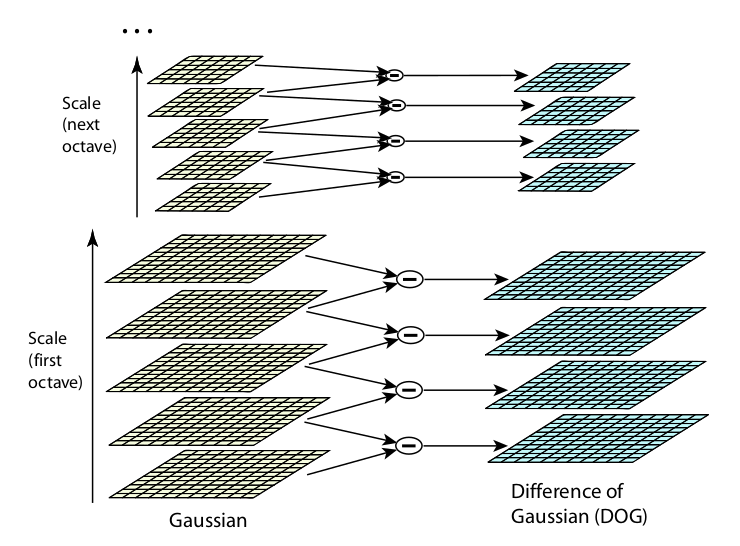
\includegraphics[width=0.6\textwidth]{sift-dog}
	\caption[Mô phỏng tính toán DoG]{Mô phỏng tính toán DoG (Nguồn:\cite{lowe2004distinctive})}
	\label{fig:sd}
\end{figure}

Các ảnh cuộn được nhóm thành các octave (mỗi octave tương ứng với giá trị gấp đôi của $\sigma$. Giá trị của $k$ được chọn sao cho số lượng ảnh mờ cho mỗi octave là cố định. Điều này đảm bảo cho số lượng các ảnh DoG cho mỗi ocvate không thay đổi.\par
Các điểm hấp dẫn được xác định là các cực đại cực tiểu của ảnh DoG qua các tỉ lệ. Mỗi điểm ảnh trong DoG được so sánh với 8 điểm láng giềng của nó ở cùng tỉ lệ đó và 9 láng giềng kề ở các tỉ lệ ngay trước và sau nó như hình \ref{fig:sle}. Nếu điểm ảnh đó đạt giá trị cực tiểu hoặc cực đại thì được chọn làm điểm hấp dẫn ứng viên.
	
\begin{figure}[h]
	\centering
	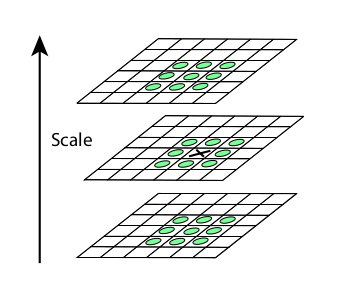
\includegraphics[width=0.4\textwidth]{sift-local-extrema}
	\caption[Quá trình tìm điểm cực trị trong hàm DoG]{Quá trình tìm điểm cực trị trong hàm DoG (Nguồn:\cite{lowe2004distinctive})}
	\label{fig:sle}
\end{figure}

\subsubsection{Định vị điểm hấp dẫn}
Loại bỏ các điểm hấp dẫn có độ tương phản thấp và các điểm hấp dẫn dọc theo các cạnh cũng được loại bỏ do không giữ được tính ổn định khi ảnh bị nhiễu như hình \ref{fig:kl} (c) sau khi đã chọn được các điểm hấp dẫn ứng viên từ hình \ref{fig:kl} (b). Các điểm còn lại sẽ được xác định hướng trong hình \ref{fig:kl} (d).\par

\begin{figure}[h]
	\centering
	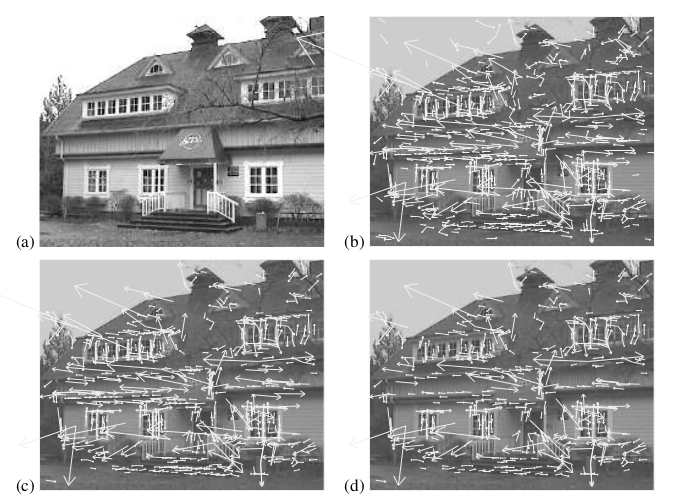
\includegraphics[width=0.7\textwidth]{keypoint-localization}
	\caption[Quá trình lựa chọn các điểm hấp dẫn]{Quá trình lựa chọn các điểm hấp dẫn (Nguồn:\cite{lowe2004distinctive}). (a) Ảnh gốc. (b) Các điểm hấp dẫn được phát hiện. (c) Sau khi loại bỏ các điểm hấp dẫn có độ tương phản thấp. (d) Sau khi loại bỏ các điểm hấp dẫn dọc theo cạnh.}
	\label{fig:kl}
\end{figure}
	
\subsubsection{Xác định hướng cho điểm hấp dẫn}
	Để xác định hướng cho điểm hấp dẫn, bằng cách tính toán biểu đồ gradient trong vùng láng giềng của điểm hấp dẫn. Độ lớn và hướng của điểm hấp dẫn được xác định theo công thức.
\begin{equation}
m(x,y) = \sqrt{(L(x+1,y) - L(x-1, y))^2 + (L(x, y+1) - L(x, y-1))^2}
\end{equation}
	
\begin{equation}
\theta(x,y) = \tan^{-1}((L(x, y+1) - L(x,y-1)) / (L(x+1, y) - L(x-1, y)))
\end{equation}	
	
\subsubsection{Mô tả các điểm hấp dẫn}
Điểm hấp dẫn sau khi được xác định hướng sẽ được biểu diễn dưới dạng các véc-tơ $4 \times 4 \times 8=128$ chiều.

\begin{figure}[h]
	\centering
	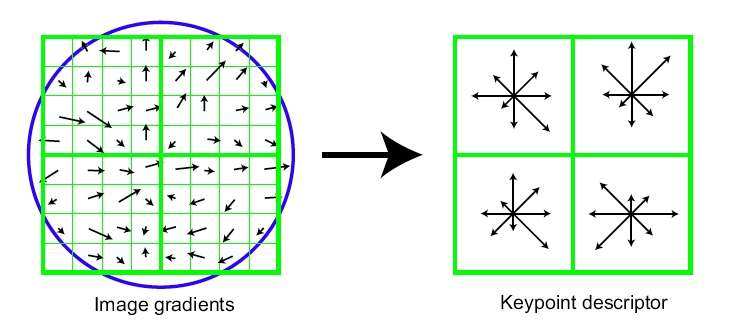
\includegraphics[width=0.7\textwidth]{keypoint-descriptor}
	\caption[Biểu diễn các vector đặc trưng]{Biểu diễn các vector đặc trưng (Nguồn:opencv-python-tutroals)}
	\label{fig:kd}
\end{figure}	


\subsubsection{Mô hình túi đựng từ trực quan}
Mô hình túi đựng từ trực quan (Bag of Visual Words - BoVW) là một khái niệm quan trọng trong chuyên ngành Khoa học máy tính, dựa trên mô hình túi đựng từ (Bag of Words - BoW) trong lĩnh vực xử lý ngôn ngữ tự nhiên (Natural Language Processing - NLP). Mô hình túi đựng từ tính toán tần số xuất hiện của từ trong tài liệu, sử dụng một biểu đồ biểu diễn tần số của từ (hình \ref{fig:histogram-visual-words}). Túi đựng từ trực quan cũng được áp dụng nguyên lý trên nhưng được xử dụng trong phân loại nội dung hình ảnh, tức là, thay thế các từ (words) thành các đặc trưng của ảnh.\par

Túi đựng từ trực quan được hiểu như là một tập các đặc trưng của một ảnh được trích chọn từ giải thuật SIFT (keypoint và descriptor) được trình bày ở phần \ref{sub:sift}, sử dụng các keypoint và descriptor này để xây dựng từ vựng.\par

\begin{figure}[h]
	\centering
	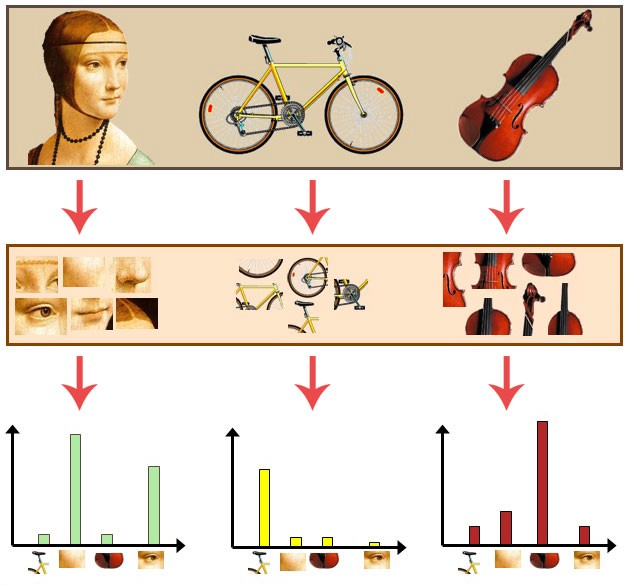
\includegraphics[width=0.5\textwidth]{histogram-visual-words}
	\caption[Biều đồ của các từ trực quan]{Biều đồ của các từ trực quan (Nguồn: towardsdatascience.com)}
	\label{fig:histogram-visual-words}
\end{figure}	

Để xây dựng một mô hình túi đựng từ trực quan. Đầu tiên, phát hiện các đặc trưng và trích xuất các mô tả (hình \ref{fig:detect-features-extracting-descriptor}) tương ứng bằng một giải thuật trích chọn đặc trưng (SIFT, KAZE, v.v.). Tiến hành gom cụm (hình \ref{fig:clustering-descriptor}) các mô tả bằng các giải thuật gom cụm (K-Means, DBSCAN, v.v.) tâm của từng cụm sẽ được sử dụng như là các từ vựng của từ điển trực quan. Tạo biểu đồ tần số dựa trên các từ vựng và tần số của các từ trong ảnh, các biểu đồ này chính là túi đựng từ trực quan (BoVW).

\begin{figure}[h]
	\centering
	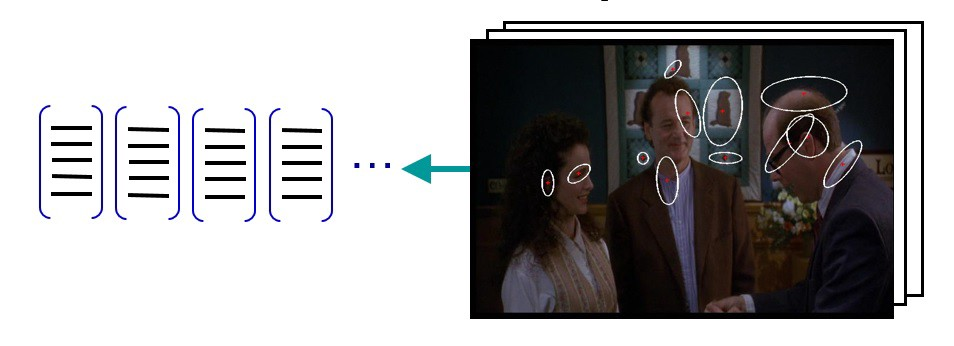
\includegraphics[width=0.7\textwidth]{detect-features-extracting-descriptor}
	\caption[Phát hiện đặc trưng và trích xuất mô tả]{Phát hiện đặc trưng và trích xuất mô tả (Nguồn: towardsdatascience.com)}
	\label{fig:detect-features-extracting-descriptor}
\end{figure}

\begin{figure}[h]
	\centering
	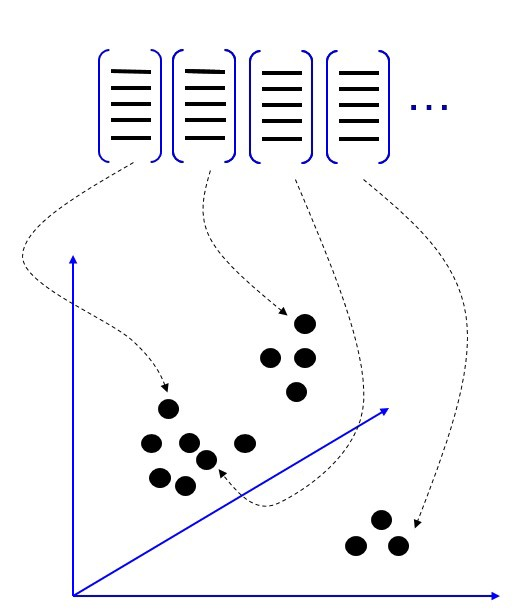
\includegraphics[width=0.4\textwidth]{clustering-descriptor}
	\caption[Gom cụm các mô tả]{Gom cụm các mô tả (Nguồn: towardsdatascience.com)}
	\label{fig:clustering-descriptor}
\end{figure}	


\subsection{Trích chọn đặc trưng Color}
Đặc trưng Color là một trong những đặc trưng phổ biến và được sử dụng nhiều trong các hệ thống tìm kiếm ảnh, được giới thiệu bởi [Michael, 1991]. Đây là phương pháp rút trích đặc trưng có nhiều ưu điểm như đơn giản, tốc độ tìm kiếm tương đối nhanh, tuy nhiên độ chính xác còn hạn chế. Một số lược đồ màu được sử dụng phổ biến như lược đồ màu RGB, HSI và HSI cải tiến. Tuy nhiên, lược đồ màu RGB được sử dụng phổ biến.  Trong phần này chúng tôi lựa chọn sử dụng lược đồ màu RGB.\par

Lược đồ màu của một hình ảnh sẽ đại diện cho sự phân bố của các thành phần màu sắc trong hình ảnh đó. Lược đồ màu sẽ được tính bằng các rời rạc hóa từng màu trong một ảnh, sau đó đếm số điểm ảnh của mỗi màu. Khi mà số lượng màu là có hạn, thuận tiện hơn là cách chuyển đổi ba 3 kênh màu (đỏ, xanh lá cây, xanh dương) thành một biến giá trị duy nhất. Một cách khác để tính lược đồ màu của ảnh RGB là phân ra làm 3 lược đồ riêng biệt $h_R$, $h_G$ và $h_B$. Khi đó, mỗi lược đồ được tính bằng cách đếm kênh màu tương ứng trong mỗi điểm ảnh.

\subsection{Trích chọn đặc trưng HOG}
Đặc trưng HOG (Histogram of Oriented Gradient) \cite{dalal2005histograms} một loại mô tả đặc trưng (feature descriptor) trừu tượng hóa đối tượng bằng cách trích xuất ra những đặc trưng của đối tượng đó và bỏ đi những thông tin không hữu ích. Đặc trưng HOG được sử dụng chủ yếu để mô tả hình dạng và sự xuất hiện của một đối tượng trong ảnh. Một mô tả đặc trưng chuyển đổi một ảnh có kích thước w$\times$h$\times$3 (channel) nhận được một vector đặc trưng có độ dài $n$.\par

Véc-tơ đặc trưng của thuật toán này khi được đưa vào mô hình máy học SVM sẽ cho ra kết quả tốt \cite{learnopencv}. Thực hiện 5 bước cơ bản để có thể xây dựng một véc-tơ đặc trưng HOG. \par

\subsubsection{Tiền xử lý}
Chuẩn hóa tỉ lệ các ảnh đầu vào theo tỉ lệ (\emph{1:2}). Ví dụ, 100$\times$200, 128$\times$256, như hình \ref{fig:hog-prep} một ảnh với kích thước 720$\times$475, chọn một đối tượng trong ảnh, tiến hành cắt đối tượng với kích thước 100$\times$200 và resize ảnh thành kích thước 64$\times$128 để tính toán mô tả đặc trưng HOG.
\begin{figure}[h]
	\centering
	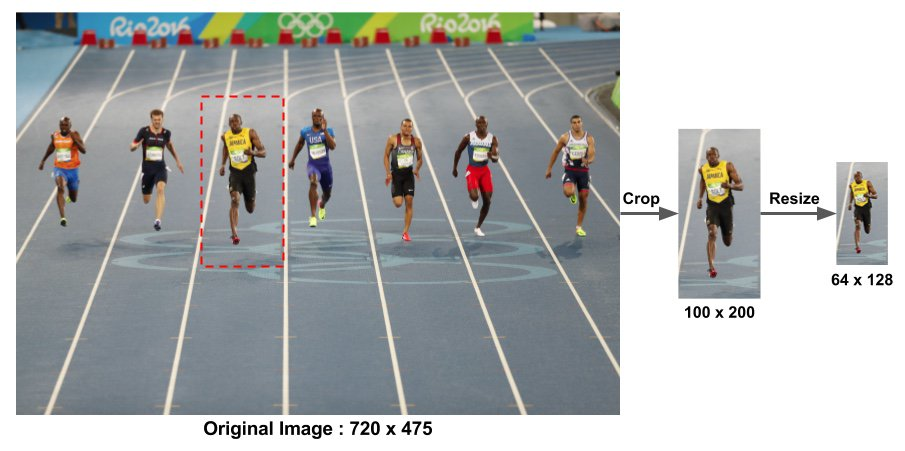
\includegraphics[width=0.8\textwidth]{hog-preprocessing}
	\caption[Tiền xử lý ảnh trong HOG]{Tiền xử lý ảnh trong HOG (Nguồn:\cite{learnopencv})}
	\label{fig:hog-prep}
\end{figure}

\subsubsection{Tính toán ảnh gradient}
Để nhận được ảnh gradient, thực hiện nhân chập (convolution) ảnh gốc \emph{I} với hai bộ lọc ảnh $d_x$ (vertical gradients) và $d_y$ (horizontal gradients).
\begin{equation}\label{eq:2.9}
 g_x = I * d_x
\end{equation}

\begin{equation}\label{eq:2.10}
 g_y  = I * d_y
\end{equation}

Tiếp tục tính toán cường độ và hướng gradient của ảnh:
\begin{equation}\label{eq:2.11}
\begin{split}
	g &= \sqrt{g_x^2 + g_y^2}\\
	\theta & = \arctan \frac{g_x}{g_x}
\end{split}
\end{equation}

Hình \ref{fig:gradient} minh họa công thức (\ref{eq:2.9}), (\ref{eq:2.10}) và (\ref{eq:2.11}).
\begin{figure}[h]
	\centering
	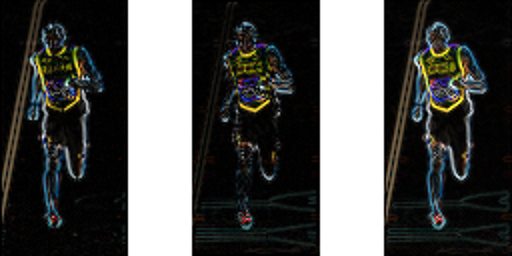
\includegraphics[width=0.8\textwidth]{gradients}
	\caption[Quá trình tính toán ảnh gradient]{Quá trình tính toán ảnh gradient (Nguồn:\cite{learnopencv}). (Left) Giá trị tuyệt đối $g_x$. (Center) Giá trị tuyệt đối $g_y$, (Right) Giá trị cường độ và hướng gradient }
	\label{fig:gradient}
\end{figure}
 
\subsubsection{Tính toán biểu đồ gradient các ô}
Để tính toán véc-tơ đặc trưng cho từng ô (cell), chia hình ảnh thành các khối (block), mỗi khối (block) lại được chia thành các ô (cell) nhỏ hơn. \par

\begin{equation}
	n_{block} = \left (\begin{array}{cc} \frac{w_{image} - w_{block} * w_{cell}}{w_{cell}} + 1 \end{array}\right) *\left (\begin{array}{cc} \frac{h_{image} - h_{block} * h_{cell}}{h_{cell}} + 1\end{array}\right)
\end{equation}

trong đó:

\begin{itemize}
	\item[-] $w_{image}, w_{block}, w_{cell}$ lần lược là chiều rộng của ảnh, khối và ô.
	\item[-] $h_{image}, h_{block}, h_{cell}$ lần lược là chiều cao của ảnh, khối và ô.
\end{itemize}

Sau khi xác định số khối và kích thước khối (block), ô (cell) để tính véc-tơ đặc trưng cho từng ô (cell), thực hiện hai bước sau:
\begin{itemize}
	\item[-] Chia không gian hướng thành \emph{b} bin (số chiều véc-tơ đặc trưng của ô).
	\item[-] Rời rạc hóa gốc hướng nghiêng tại mỗi điểm ảnh trong các bin.
\end{itemize}

Giả sử gốc nghiêng tại vị trí ($x, y$) có độ lớn $\alpha(x,y)$.
\begin{itemize}
	\item[-] Trường hợp rời rạc hóa unsigned, $b = 9$.
	\begin{equation}
		B(x,y) = round(\frac{b*\alpha(x,y)}{\pi}) \bmod b 
	\end{equation}
	
	\item[-] Trường hợp rời rạc hóa signed, $b = 18$.
	\begin{equation}
		B(x,y) = round(\frac{b*\alpha(x,y)}{2\pi}) \bmod b
	\end{equation}
\end{itemize}

Giá trị bin được định lượng bởi tổng cường  độ biến thiên của các điểm ảnh (pixel) thuộc về bin đó. Tập các véc-tơ của ô sẽ được nối thành véc-tơ đặc trưng khối theo công thức:
\begin{equation}
	size_{block} = n * size_{cell}
\end{equation}

trong đó:

\begin{itemize}
	\item[-] $n$ là số khối
	\item[-] $size_{cell}$ là số chiều véc-tơ đặc trưng ô
\end{itemize}

Như hình \ref{fig:hog-prep} có kích thước 64$\times$128 sẽ được chia thành các khối có kích thước 16$\times$16. Mỗi khối gồm 4 ô, mỗi ô có kích thước 8$\times$8 như hình \ref{fig:hog-cells}.
\begin{figure}[h]
	\centering
	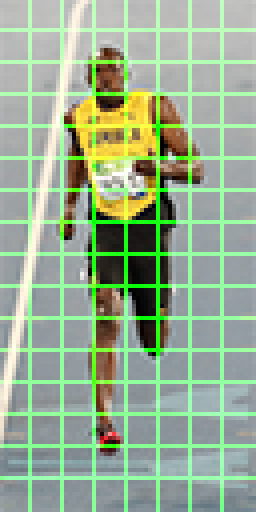
\includegraphics[width=0.2\textwidth]{hog-cells}
	\caption[Chia ảnh thành các block 16$\times$16]{Chia ảnh thành các block 16$\times$16 (Nguồn:\cite{learnopencv})}
	\label{fig:hog-cells}
\end{figure}
Tính toán đặc trưng HOG tại mỗi cell ở trương hợp rời rạc hóa với $b=9$. Hướng gradient chạy trong khoảng $0 - 180^{\circ}$, trung bình $20^{\circ}$ mỗi bin.\par

Tại mỗi ô, xây dựng một biểu đồ cường độ gradient bằng cách bình chọn điểm ảnh vào biểu đồ. Trọng số bình chọn của mỗi điểm ảnh phụ thuộc vào hướng và cường độ gradient của điểm ảnh đó, được mô tả trong hình \ref{fig:hog-cell-gradients}.
\begin{figure}[h]
	\centering
	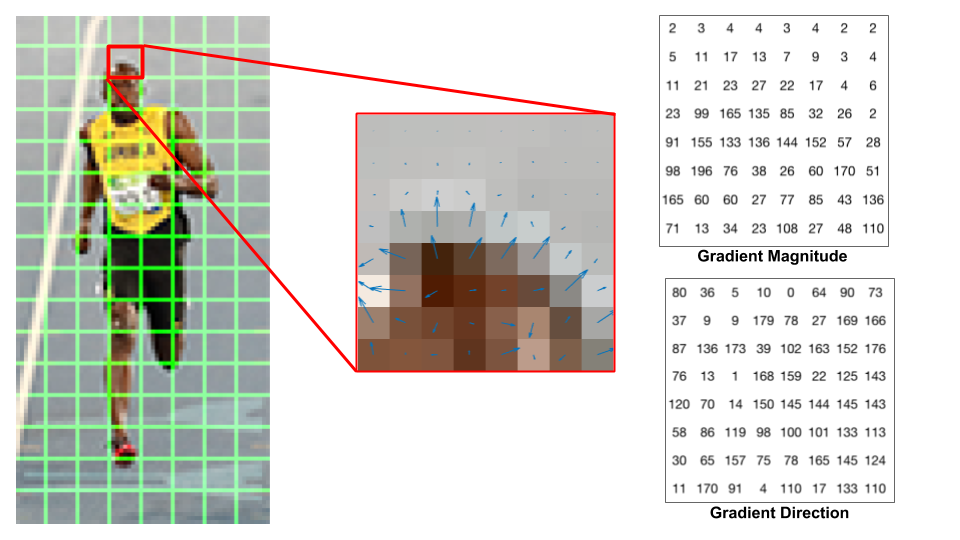
\includegraphics[width=0.8\textwidth]{hog-cell-gradients}
	\caption[Tính toán biểu đồ gradient]{Tính toán biểu đồ gradient (Nguồn:\cite{learnopencv})}
	\label{fig:hog-cell-gradients}
\end{figure}

Tại vị trí điểm ảnh đầu tiên, sẽ có hướng $80^{\circ}$ và giá trị cường độ là 2, sẽ được thêm vào vị trí bin thứ 5. Tại vị trí pixel thứ 4 có hướng $10^{\circ}$ và giá trị cường độ là 4, do không có bin với hướng $10^{\circ}$ nên giá trị cường độ được chia 2 và thêm vào bin 1 và 2 trong hình \ref{fig:hog-histogram-1}.
\begin{figure}[h]
	\centering
	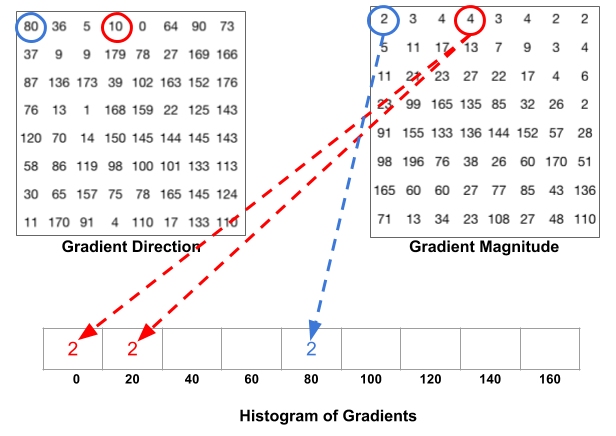
\includegraphics[width=0.8\textwidth]{hog-histogram-1}
	\caption[Bình chọn điểm ảnh vào biểu đồ]{Bình chọn điểm ảnh vào biểu đồ (Nguồn:\cite{learnopencv})}
	\label{fig:hog-histogram-1}
\end{figure}

\subsubsection{Chuẩn hóa các khối}
Do gradient của ảnh nhạy cảm với độ sáng, việc bình thường hóa biểu đồ (histogram) để gradient không bị ảnh hưởng từ những thay đổi ánh sáng trong ảnh. Gọi $I_{01}$ là một vector màu [128, 64, 32], độ dài của véc-tơ $I_{01}$ là $\sqrt{128^2 + 64^2 + 32^2} = 146. 64$, chia từng phần tử [128, 64, 32] cho 146.64 nhận được một véc-tơ chuẩn hóa [0.87, 0.43, 0.22]. $I_{02}$ là một véc-tơ màu [256, 128, 64] thực hiện các bước tiếp theo tương tự như $I_{01}$ ban đầu ta vẫn nhận được một véc-tơ chuẩn hóa giống $I_{01}$.\par

Để chuẩn hóa 1 biểu đồ (histogram) có số bin là $b = 9$, không thể áp dụng như cách chuẩn hóa một véc-tơ (3$\times$1) đã nêu.  Chuẩn hóa một khối kích thước 16$\times$16 tương ứng mỗi khối sẽ có 4 biểu đồ (histograms) tức là, tương ứng 4 ô sẽ là 1 biểu đồ, mỗi 1 histogram có kích thước 9$\times$1 nối 4 biểu đồ lại tạo thành một véc-tơ phần tử 36$\times$1, véc-tơ phần tử này có thể được chuẩn hóa theo cách một véc-tơ 3$\times$1 được chuẩn hóa.

\subsubsection{Tính toán véc-tơ đặc trưng}
Với mỗi ảnh kích thước 64$\times$128, chia thành các khối 16$\times$16 chồng nhau, sẽ có 7 khối theo chiều ngang và 15 khối theo chiều dọc. Như vậy số khối nhận được là $7 \times 5=105$. Mỗi khối gồm 4 ô, khi áp dụng biểu đồ có số bin là $b=9$ cho mỗi ô, mỗi khối sẽ được đại diện bởi một véc-tơ có kích thước 36$\times$1. Khi nối của tất cả khối lại với nhau, thu được véc-tơ đặc trưng HOG có kích thước $105 \times 36 \times 1 =$ 3780$\times$1.


\subsection{Trích chọn đặc trưng GIST}
Đặc trưng GIST là đặc trưng toàn cục biểu diễn nội dung của một ảnh được giới thiệu bởi [Oliva \& Torralba, 2004]. Ý tưởng chính là xây dựng một mô tả ở mức hấp dẫn của ngữ cảnh trong ảnh, mà không yêu cầu một hình thức phân đoạn nào, nghiên cứu đã đề xuất một tập hợp các đặc trưng quan trọng như tính tự nhiên (degree of naturalness), tính mở rộng (degree of expansion), độ nhám (degree of roughness), tính cởi mở (degree of openness), độ chắc chắn (degree of ruggedness). Tập hợp này cho phép trình bày cấu trúc không gian của một ngữ cảnh trong ảnh. Đặc trưng mô tả toàn cục GIST hiện nay đã cho kết quả tốt trong việc tìm kiếm ảnh [Douze et al., 2009], phân lớp ảnh, nhận dạng chữ viết tay [Do \& Pham, 2015]. Quá trình trích chọn đặc trưng GIST được thực hiện như sau:\par

\subsubsection{Tiền xử lý ảnh}
Chuẩn hóa kích thước ảnh về n$\times$m sao cho có thể chia ảnh thành w$\times$h vùng bằng nhau. Phép biến đổi Fourier được sử dụng khi trích đặc trưng GIST, vì thế kích thước của ảnh phải được chuẩn hóa về dạng n$\times$m $=2^n \times 2^n$. Tiếp theo, tách ảnh thành ba kênh màu riêng biệt (đỏ, xanh lá cây, xanh dương) đối với ảnh màu để thực hiện phép biến đổi cho từng kênh màu. Cuối cùng, biến đổi ảnh mức xám mục đích cho ra ảnh có giá trị mức xám thấp được mở rộng và các giá trị mức xám cao bị nén lại.

\subsubsection{Sinh bộ lọc Gabor}
Bộ lọc Gabor được sử dụng rộng rải khi phân tích dữ liệu. Trong lĩnh vực xử lý ảnh, phương pháp này thường được dùng để trích đặc trưng hay phân đoạn ảnh kết cấu và có độ chính xác cao. Trong các ứng dụng phân tích kết cấu ảnh, thông thường bộ lọc Gabor được sử dụng theo một thang lọc. Mỗi thang lọc thực hiện cho một tần số và đồng thời lọc theo nhiều ứng dụng khác nhau. Trong việc trích chọn đặc trưng này, chúng tôi sử dụng 20 bộ lọc Gabor bao gồm 3 thang lọc và 8 hướng. Trong đó, thang 1 và 2 gồm 8 bộ lọc và thang 3 gồm 4 bộ lọc. Công thức sinh dãy bộ lọc gabor được thể hiện như sau:
\begin{equation}
G(u, v) = e^{-10*0.35*(\frac{f_r(u, v)}{Nf_s}-1)^2 - 2 \pi p \delta_\theta^2}
\end{equation}

trong đó, \par
\begin{itemize}

\item[-] $f_r(u,v)$ là giá trị chuẩn hóa bán kính tần số, được tính theo công thức (\ref{eq:2.17}) và (\ref{eq:2.18}):
\begin{equation}\label{eq:2.17}
f_r(f_x, f_y) = \sqrt{f_x(x, y)^2 + f_y(x, y)^2} 
\end{equation}

\begin{equation}\label{eq:2.18}
f_r(u, v) = shift(f_r(f_x, f_y))
\end{equation}

\item[-] $N$: kích thước của bộ lọc (bằng kích thước ảnh\par
\item[-] $f_s$: tần số ứng với từng thang $f_s = k^{-s}f_{max}$ với, $f_{max} = 0.3$ là tần số cực đại\par
\item[-] $p$: băng thông của bộ lọc $p = \frac{16*O_s^2}{N^2}$ với, $O_s$ là số hướng ứng với từng than $s$
\item[-] $\delta_\theta$: hướng của bộ lọc với, $\theta = n\frac{\pi}{O}n=0, 1, \dots, O-1$
\end{itemize}

\subsubsection{Tính toán véc-tơ đặc trưng}
%\begin{itemize}
\emph{Biến đổi Fourier rời rạc  -- Discrete Fourier Transform (DFT)}.
Phép biến đổi Fourier được dùng nhiều trong xử lý tín hiệu số. Vì ảnh kỹ thuật số là môt phần của tín hiệu số nên phải dùng dạng khác của biến đổi Fourier, đó là biến đổi Fourier rời rạc. Biến đổi DFT được triển khai hai chiều của một ảnh kích thước n$\times$m, xác định bởi một cặp biến đổi:
\begin{itemize}
\item[-] Biến đổi Fourier rời rạc thuận (DFT), chuyển đổi từ miền không gian $f(x,y)$ sang miền tần số $F(x,y)$.
\item[-] BIến đổi Fourier rời rạc ngược (IDFT), chuyển đổi ảnh từ miền tần số $F(x,y)$ sang miền không gian $f(x,y)$
\end{itemize}

\emph{Áp dụng bộ lọc Gabor}.
Trước tiên thực hiện phép biến đổi Fourier thuận trên từng ảnh ứng với từng thành phần màu đã được tiền xử lý để chuyển đổi ảnh vè miền tần số (\ref{eq:2.19}). Gọi $i = 1, 2, \dots, 20$ là số bộ lọc Gabor được áp dụng lên từng ảnh màu bằng cách nhân giá trị của bộ lọc Gabor với giá trị phức của từng ảnh tại vị trí $(u,v)$ tương ứng công thức (\ref{eq:2.20}). Công thức (\ref{eq:2.21}) thực hiện phép biến đổi Fourier ngược lên từng ảnh để chuyển đổi miền không gian, dựng lại ảnh và trích đặc trưng. \par

\begin{equation}\label{eq:2.19}
F_{R, G, B}(u, v) = DFT[f_{R, G, B}(x,y)]
\end{equation}

\begin{equation}\label{eq:2.20}
G_{R, G, B}(u,v) = Gabor_i(u, v) * F_{R, G, B}(u, v)
\end{equation}

\begin{equation}\label{eq:2.21}
\begin{split}
g_{R, G, B} &= IDFT[G_{R, G, B}(u,v)]\\
f_{R, G, B}(x, y) & = \sqrt{g_{R, G, B_{real}}(x, y)^2 + g_{R, G, B_{imaginary}}(x, y)^2}
\end{split}
\end{equation}


\emph{Chia vùng và trích đặc trưng}. 
Sau khi ảnh được áp dụng qua 20 bộ lọc Gabor và phép biến đổi Fourier ngược sẽ tiến hành trích đặc trưng. Để trích đặc trưng, trước hết cần chia ảnh thành 16 vùng phân biệt có kích thước bằng nhau, rồi trích đặc trưng trên mỗi vùng dựa vào công thức (\ref{eq:2.22}). Ghép vector đặc trưng của từng vùng lại với nhau để nhận được vector đặc trưng của ảnh. Công thức (\ref{eq:2.23}) xác định số chiều của vector đặc trưng.

\begin{equation}\label{eq:2.22}
d_i = \frac{\sum \text{\emph{Giá trị các điểm ảnh thuộc vùng i}}}{\sum \text{\emph{Số lượng điểm ảnh của vùng i}}}
\end{equation}

\begin{equation}\label{eq:2.23}
n_D = n_R * n_{Gabor} * W^2
\end{equation}

trong đó,
\begin{itemize}
\item[-] $n_D$ là số chiều của vector đặc trưng
\item[-] $n_R$ là số thành phần màu sử dụng để biểu diễn cho mỗi điểm ảnh
\item[-] $n_{Gabor}$ là số lượng bộ lọc áp dung lên mỗi kênh màu
\item[-] $W^2$ là số vùng phân biệt có kích thước bằng nhau được chia ra từ ảnh
\end{itemize}
%\end{itemize}


\subsection{Trích chọn đặc trưng sử dụng mạng nơ-ron tích chập}
\subsubsection{Tổng quan mạng nơ-ron tích chập}
Mạng nơ-ron tích chập (Convolutional Neural Network - CNNs) là một trong những mô hình học sâu tiên tiến, được sử dụng nhiều trong các bài toán nhận dạng các đối tượng trong ảnh. \par

Kiến trúc mạng nơ-ron tích chập chung thông thường sẽ có cấu trúc hai phần. Đầu tiên, phần học đặc trưng (feature learning). Thứ hai, là phần phân lớp (classification). Một ảnh đầu vào (input layer) sẽ được nhân chập với lớp convolutional (convolutional layer), đầu ra của lớp convolutional sẽ đi qua hàm kích hoạt (activation) theo sau là một lớp pooling (pooling layer) mục đích giảm kích thước dữ liệu tại phần học đặc trưng. Sau khi qua lớp convolutional và lớp pooling, kết quả tại phần học đặc trưng sẽ được làm phẳng thành một véc-tơ cột, dùng lớp fully connected (fully connected layer) để kết nối các đặc điểm của ảnh để nhận được một lớp đầu ra (output layer) được mô tả trong hình \ref{fig:cnn-architecture}.

\begin{figure}[h]
	\centering
	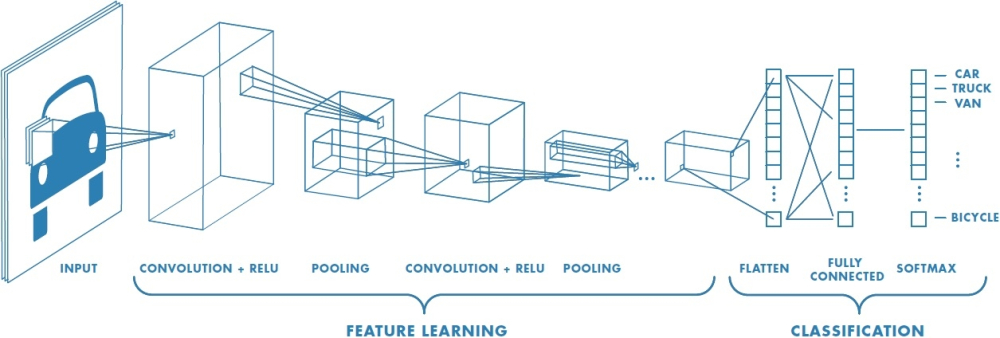
\includegraphics[width=0.8\textwidth]{cnn-architecture}
	\caption[Kiến trúc mạng nơ-ron tích chập]{Kiến trúc mạng nơ-ron tích chập (Nguồn: anhvnn.wordpress.com)}
	\label{fig:cnn-architecture}
\end{figure}

\begin{itemize}
\item[-] \emph{Lớp convolutional} (convolutional layer) còn được biết đến như là một cửa sổ trượt (sliding window), nhân (kernel) hay bộ lọc (filter) như hình \ref{fig:convolve}. Một ảnh nhị phân (trắng đen) \emph{I} được biểu diễn dưới dạng một ma trận 2 chiều, một cửa sổ trượt \emph{K} được biểu diễn bằng một ma trận 2 chiều (kích thước 3$\times$3). Thực hiện phép tích chập ($I*K$) giữa ảnh \emph{I} và cửa sổ trượt \emph{K} bằng cách di chuyển cửa sổ trượt theo số bước trượt (stride -- \emph{thường được dùng để giảm kích thước của ảnh đầu vào, sau phép nhân tích chập}) được chỉ định từ trái sang phải và từ trên xuống dưới. Kết quả thu được một ma trận $I$' có kích thước nhỏ hơn ma trận $I$, tức là ($I$'$<  I$). Để nhận được một ma trận $I$' có cùng kích thước với $I$ ta thực hiện nhân tích chập với tham số $padding = k$ (zero-padding) sẽ thêm \emph{k} véc-tơ giá trị 0 vào viền ngoài của ma trận ảnh $I$. Dễ dàng tính toán lớp đầu ra bằng công thức (\ref{eq:2.24}).\par
\begin{equation}\label{eq:2.24}
\frac{N_I - F_K + 2P}{S} + 1
\end{equation}
trong đó,
\begin{itemize}
\item $N_I$ là kích thước ảnh đầu vào
\item $F_K$ là kích thước cửa sổ trượt 
\item $P$ là giá trị của zero-padding
\item $S$ là giá trị của bước trượt
\end{itemize}

\begin{figure}[h]
	\centering
	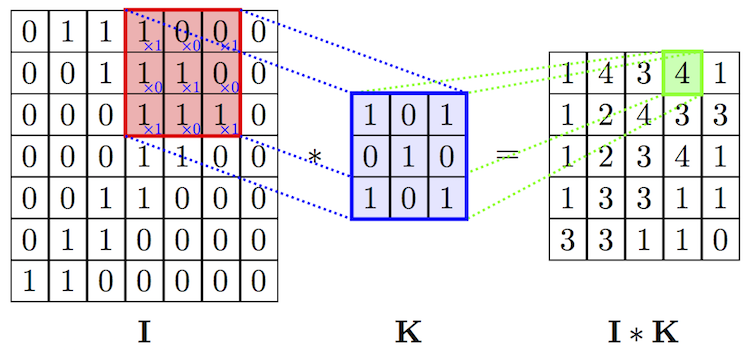
\includegraphics[width=0.7\textwidth]{convolve}
	\caption[Nhân tích chập ảnh \emph{I} và cửa sổ trượt \emph{K}]{Nhân tích chập ảnh \emph{I} và cửa sổ trượt \emph{K} (Nguồn: anhvnn.wordpress.com)}
	\label{fig:convolve}
\end{figure}

\item[-] \emph{Lớp pooling} (pooling layer).
Lớp pooling thường được dùng giữa các lớp convolutional, giảm kích thước dữ liệu đầu vào (ảnh \emph{I}) nhưng giữ được các thông tin quan trọng làm giảm việc tính toán cho mô hình phân lớp. Sau khi kết quả đầu ra của convolutional đi qua hàm activation, mỗi một activation sẽ được biến đổi bằng hàm kích hoạt phi tuyến ReLU như hình \ref{fig:cnn-architecture}, nếu sử dụng max-pooling kích thước 2$\times$2 (pooling-size), $stride = 2$ thì nhận được một ảnh có kích thước bằng một nữa ảnh đầu vào như hình \ref{fig:pooling-layer}. Max-pooling được sử dụng thông dụng hiện nay sẽ lấy giá trị cao nhất trong pooling-size kích thước 2$\times$2, còn average-pooling sẽ lấy giá trị trung bình.

\begin{figure}[h]
	\centering
	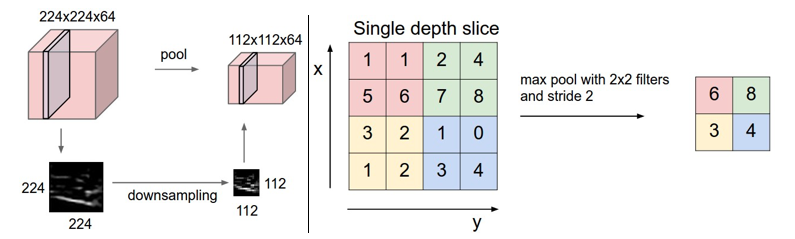
\includegraphics[width=0.8\textwidth]{pooling-layer}
	\caption[Lớp pooling giảm kích thước dữ liều đầu vào]{Lớp pooling giảm kích thước dữ liều đầu vào (Nguồn: anhvnn.wordpress.com)}
	\label{fig:pooling-layer}
\end{figure}

\item[-] \emph{Lớp fully-connected} (fully-connected layer).
Sau khi qua các lớp convolutional và lớp pooling thì mô hình đã học được tương đối nhiều đặc điểm của ảnh, đầu ra cuối cùng này sẽ là được làm phẳng (hình \ref{fig:flattern}) thành một véc-tơ cột trước khi dùng lớp fully-connected để kết nối các đặc điểm của ảnh để ra được output của model (hình \ref{fig:fully-connected}).\par

\begin{figure}[h]
	\centering
	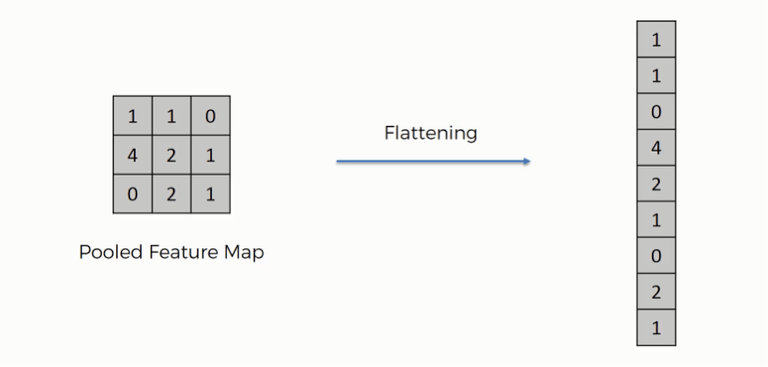
\includegraphics[width=0.6\textwidth]{flattern}
	\caption[Làm phẳng output của lớp cuối cùng]{Làm phẳng output của lớp cuối cùng (Nguồn: nttuan8.com)}
	\label{fig:flattern}
\end{figure}

\begin{figure}[h]
	\centering
	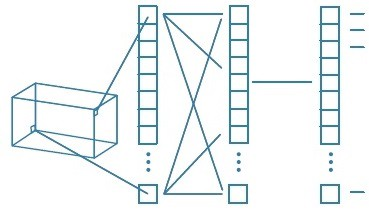
\includegraphics[width=0.4\textwidth]{fully-connected}
	\caption[Làm phẳng lớp cuối cùng và kết nối đến fully-connected]{Làm phẳng và kết nối đến fully-connected (Nguồn: anhvnn.wordpress.com)}
	\label{fig:fully-connected}
\end{figure}

\end{itemize}


\subsubsection{Mô hình Residual Networks}
Để tăng độ chính xác khi huấn luyện cho các mô hình mạng nơ-ron tích chập, bằng cách tăng số lượng layer, nhưng nếu số lượng layer lớn (trên 50) sẽ gặp tình trạng gradient của hàm mất mát quá nhỏ hoặc quá lớn do thuật toán lan truyền ngược được gọi lần lượt là vanishing gradients đối với mạng nơ-ron sâu (Deep Neural Networks) và exploding gradients đối với mạng nơ-ron hồi quy (Recurrent Neural Networks) làm cho mô hình khó hội tụ. Mô hình Residual Networks (ResNet)  [He et al., 2015] \cite{He2015} được ra đời để giải quyết các vấn đề của các mô hình máy học truyền thống. \par

Mô hình ResNet là mô hình chiến thắng trong cuộc thi \emph{ImageNet Large Scale Visual Recognition Challenge 2015} (ILAVRC2015). Sử dụng đến 152 layers -- sâu hơn 8 lần so với mô hình VGG, chỉ số lỗi nhận được trên tập dữ liệu kiểm tra của ImageNet  là 3.57\%. Để giải quyết vấn đề vanishing và exploling bằng cách thêm một \emph{batch normalization} trước mỗi activation cho mỗi layer có nhiệm vụ chuẩn hóa dữ liệu đầu ra, các hệ số trở nên cân bằng giúp mô hình dễ dàng hội tụ. Một vấn đề nữa được nêu trong \cite{He2015} là vấn đề bão hòa độ chính xác của mô hình (degradation), tức là, độ chính xác của mô hình không tăng khi thêm nhiều layer hơn hoặc không giảm khi ít layer, đây không phải là hiện tượng overfitting mà do mô hình càng sâu thì càng khó huấn luyện, vấn đề được tác giả và cộng sự của ông giải quyết bằng cách cứ mỗi 2 layers cộng input với output, được gọi là \emph{residual block}. Kiến trúc của ResNet gồm nhiều \emph{residual block} được tính theo công thức $H(x) = F(x) + x$ mô hình sẽ dễ dàng hội tụ hơn như trong hình \ref{fig:residual-block}.\par

\begin{figure}[h]
	\centering
	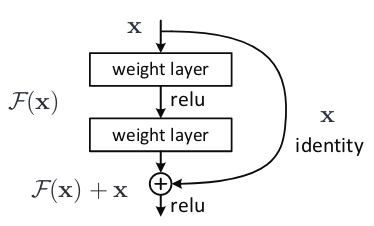
\includegraphics[width=0.5\textwidth]{residual-block}
	\caption[Residual block]{Residual block (Nguồn: anhvnn.wordpress.com)}
	\label{fig:residual-block}
\end{figure}


\section{Máy học véc-tơ hỗ trợ}
\subsection{Giới thiệu}
Máy học véc-tơ hỗ trợ (Support Vector Machines - SVM) [Vapnik, 1995] là một mô hình phân lớp nhị phân tuyến tính (học có giám sát), phân lớp được xác định bởi một siêu phẳng tách biệt, thuật toán đi tìm một siêu phẳng tối ưu.\par

Xét ví dụ phân lớp nhị phân tuyến tính đơn giản \cite{khang2019} được mô tả như hình \ref{fig:2.10} với \emph{m} phần tử $x_1, x_2, \dots, x_n$ trong không gian \emph{n} chiều với nhãn (lớp) của các phần tử tương ứng là $y_1, y_2, \dots, y_n$ có giá trị là \emph{1} (lớp dương) hay \emph{-1} (lớp âm). Giải thuật SVM [Vapnik, 1995] tìm một siêu phẳng tối ưu (xác định bởi véc-tơ pháp tuyến $w$ và độ lệch của siêu phẳng với tọa độ $b$) để tách dữ liệu ra hai lớp. Giải thuật SVM tìm siêu phẳng tách biệt hai lớp ra xa nhất có thể (siêu phẳng tối ưu) dựa trên hai siêu phẳng hỗ trợ song song của hai lớp. Siêu phẳng hỗ trợ của lớp $+1$ ($w.x - b = +1$) là siêu phẳng của phần tử $x_p$ thuộc lớp $y_p = +1$ nằm về phía bên phải của nó, tức là: $w.x_p - b \geq +1$. Tương tự siêu phẳng hỗ trợ của lớp $-1$ ($w.x - b = -1$) là các siêu phẳng mà các phần tử $x_n$ thuộc lớp $y_n = -1$ nằm về phía bên trái của siêu phẳng của nó, tức là: $w.x_n - b \leq +1$. Những phần tử nằm ngược phía với siêu phẳng hỗ trợ được coi như lỗi. Khoảng cách được biểu diễn bởi $z_i \geq 0$ (với $x_i$ nằm đúng phía của siêu phẳng hỗ trợ của nó thì khoảng cách lỗi tương ứng $z_i = 0$, ngược lại $z_i > 0$ là khoảng cách từ điẻm $x_i$ đến siêu phẳng hỗ trợ tương ứng của nó). Khoảng cách giữa hai siêu phẳng hỗ trợ gọi là lề $= 2/\|w\|$, trong đó $\|w\|$ là độ lớn ($2-corm$) của vector pháp tuyến $w$. Siêu phẳng tối ưu (nằm giữa hai siêu phẳng hỗ trợ) cần tìm phải được cực đại hóa lề (lề càng lớn, mô hình phân lớp càng an toàn) và cực tiểu lỗi. Vấn đề tìm siêu phẳng tối ưu của giải thuật SVM dẫn đến việc giải quyết bài toán quy hoạch toàn phương (2.42).

\begin{figure}[h]
	\centering
	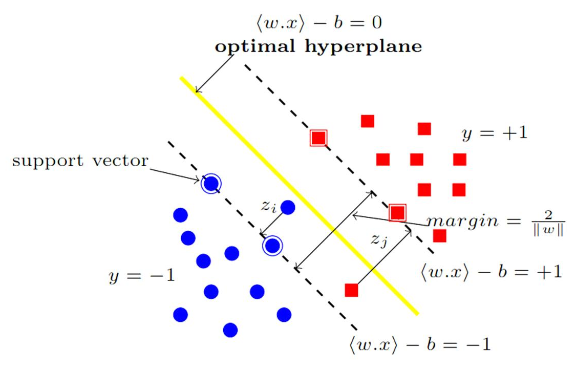
\includegraphics[width=0.6\textwidth]{svm-model}
	\caption[Phương pháp tuyến tính với máy học SVM]{Phương pháp tuyến tính với máy học SVM (Nguồn: NCKH)}
	\label{fig:2.10}
\end{figure}

\begin{equation}\label{eq:svm}
	\begin{aligned}
		\min_{\alpha}\frac{1}{2} \sum_{i=0}^m \sum_{j=0}^m y_i y_j \alpha_i \alpha_j K \langle x_i x_j \rangle - \sum_{i=1}^m \alpha_i \\
		\text{với ràng buộc}:
		\begin{cases} 
			\displaystyle\sum_{i=1}^m y_i \alpha_i = 0\\
			0 \leq \alpha_i \leq \boldsymbol{C} & \forall i = 1,2, \dots, m
		\end{cases}
	\end{aligned}
\end{equation}

Trong đó $\boldsymbol{C}$ là hằng số thường dùng để điều chỉnh độ rộng của lề phân hoạch và tổng khoảng cách lỗi; $K\langle x_i, x_j\rangle$ là hàm nhân tuyến tính $K \langle x_i, x_j \rangle = \langle x_i \bullet x_j \rangle$.\par

Giải bài toán huy hoạch toàn phương (\ref{eq:svm}) thu được \emph{\#LC} phần tử $x_i$ tương ứng với $x_i > 0$, được gọi là vector hỗ trợ. Chỉ cần \emph{\#LC} hỗ trợ này ta có thể dựng lại được siêu phẳng phân lớp. Mô hình SVM thực hiện phân lớp phần tử mới \emph{x} bằng (\ref{eq:predict})

\begin{equation}\label{eq:predict}
predict(x) = sign \left( \sum_{i=1}^{\#LC} y_i \alpha_i K\langle x, x_i \rangle - b \right)
\end{equation}

Máy học vector hỗ trợ có thể sử dụng các hàm nhân khác nhau để giải quyết lớp các bài toán phân lớp phi tuyến [Cristianini \& Shawe-Taylor, 2000]. Để xử lý các vấn đề phân lớp phi tuyến, không cần bất kỳ thay đổi nào hơn từ giải thuật mà chỉ cần thay thế hàm nhân tuyến tính trong (\ref{eq:svm}) và (\ref{eq:predict}) bằng các hàm nhân khác. Hàm phi tuyến phổ biến là hàm cơ sở bán kính (Radial Basic Function -- RBF): $\boldsymbol{K} \langle x_i, x_j \rangle = e^{-\gamma\|x_i - x_j\|^2}$ 

Mô hình máy học SVM cho kết quả cao, ổn định, chịu đựng nhiễu tốt và phù hợp với các bài toán phân lớp, hồi quy. Nhiều ứng dụng thành công của SVM đã được công bố trong nhiều lĩnh vực như nhận dạng ảnh, phân loại văn bản và sinh-tin học [Guyon, 1999].

Đề giải quyết vấn đề phân lớp đa lớp (số lớp $c \geq 3$), giải thuật SVM thường mở rộng theo 2 phương pháp đơn giản là 1-vs-all [Vapnik, 1995] và 1-vs-1 [Krebel, 1999].

\begin{figure}[h]
	\centering
	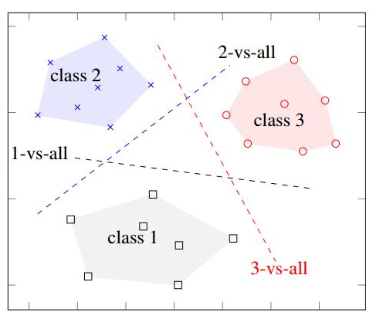
\includegraphics[width=0.4\textwidth]{one-vs-all}
	\caption[Phương pháp 1-vs-all cho máy học SVM đa lớp]{Phương pháp 1-vs-all cho máy học SVM đa lớp (Nguồn: \cite{khang2019})}
	\label{fig:2.11}
\end{figure}

\begin{figure}[h]
	\centering
	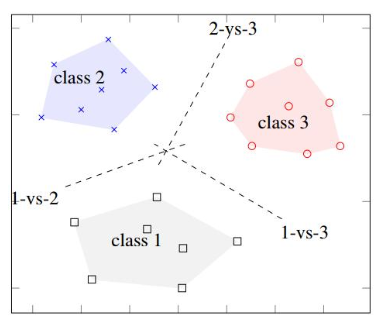
\includegraphics[width=0.4\textwidth]{one-vs-one}
	\caption[Phương pháp 1-vs-1 cho máy học SVM đa lớp]{Phương pháp 1-vs-1 cho máy học SVM đa lớp (Nguồn: \cite{khang2019})}
	\label{fig:2.12}
\end{figure}

Phương pháp 1-vs-all (hình \ref{fig:2.11}) xây dựng $c$ mô hình SVM nhị phân, mô hình $c_i$ tách lớp $c_i$ (lớp dương) ra khỏi các lớp khác (âm). Phương pháp 1-vs-1 (hình \ref{fig:2.12}) xây dựng $c(c-1)/2$ mô hình SVM nhị phân, mỗi mô hình tách một cặp 2 lớp. Việc phân lớp dựa vào bình phương chọn khoảng cách đến các siêu phẳng thu được từ SVM nhị phân.


\subsection{Ưu điểm}
Điểm nỗi bậc của giải thuật SVM là đồng thời cực tiểu hóa lỗi phân lớp và cực đại hóa khoảng cách lề giữa các lớp, từ đó tối ưu hóa hiệu suất phân lớp kể cả khi không gian đặc trưng có số chiều lớn. Ngoài ra, thời gian phân lớp của giải thuật SVM cũng khá nhanh.

\subsection{Nhược điểm}
Đối với giải thuật SVM để đạt được kết quả phân loại tốt cần chọn hàm nhân phù hợp. Ngoài ra, đối với bài toán phân lớp đa lớp, giải thuật SVM phải lặp đi lặp lại quá trình huấn luyện vì SVM chỉ giải quyết bài toán phân lớp nhị phân. Do đó cần rất nhiều thời gian để giải thuật SVM huấn luyện mô hình.











